% !TEX encoding = UTF-8 Unicode
% !TEX TS-program = pdflatex
% !TEX encoding = UTF-8 Unicode
% !TEX root = tabelle.primo.tex
	\chapter{Numeri Naturali}
\label{cha:NumeriNaturali}
\minitoc
\mtcskip                                % put some skip here
\minilof                                % a minilof
\mtcskip                                % put some skip here
\minilot
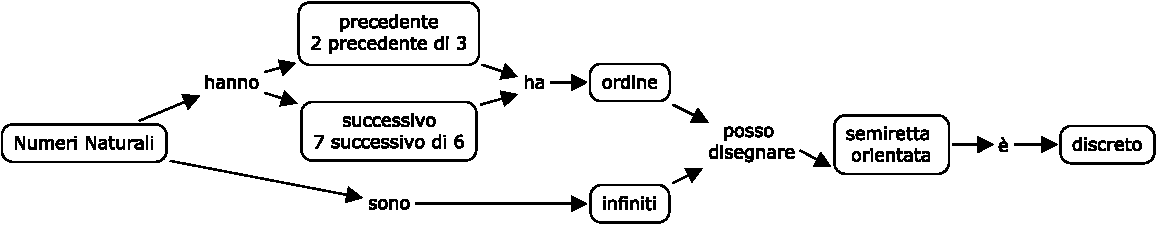
\includegraphics[scale=0.80]{NumeriNaturali-crop}
\section{Addizione}
\label{sec:NumerinatADD}
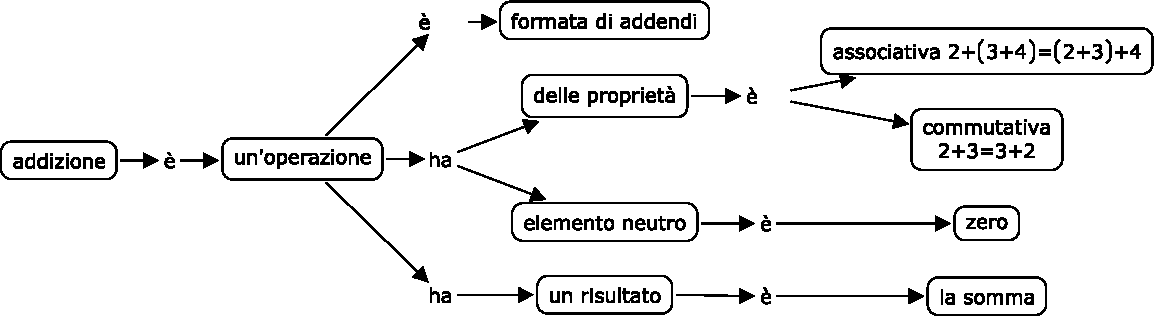
\includegraphics[scale=0.80]{Numerinaturali_somma-crop}
\section{Sottrazione}
\label{sec:NumerinatDiff}
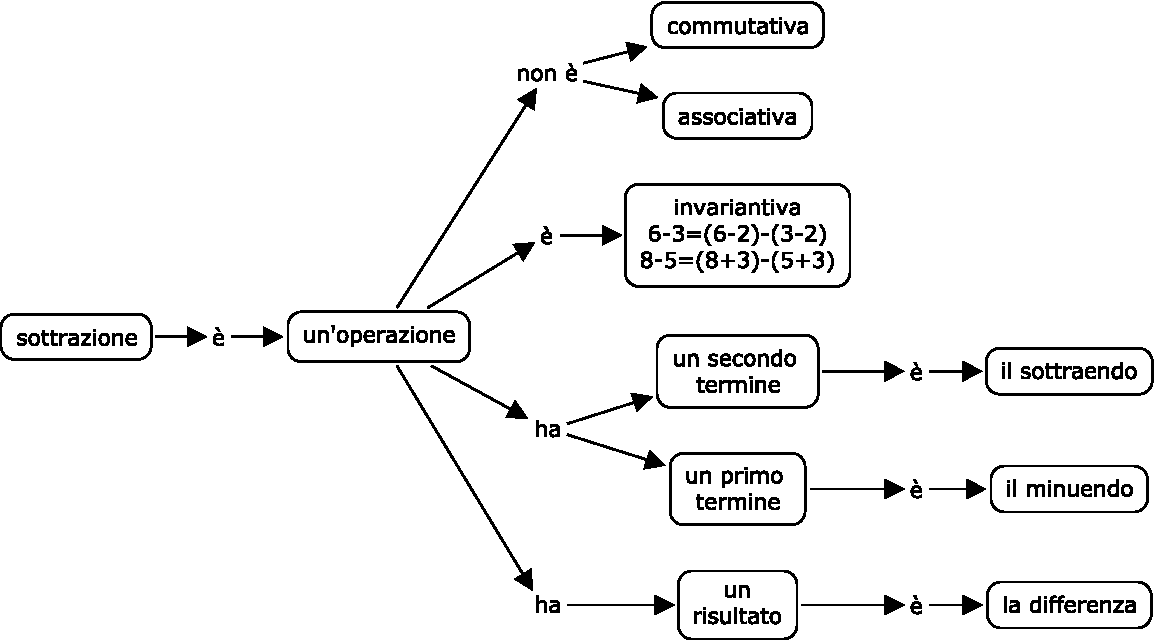
\includegraphics[scale=0.80]{Numerinaturali_differenza-crop}
\section{Moltiplicazione}
\label{sec:NumerinatMolt}
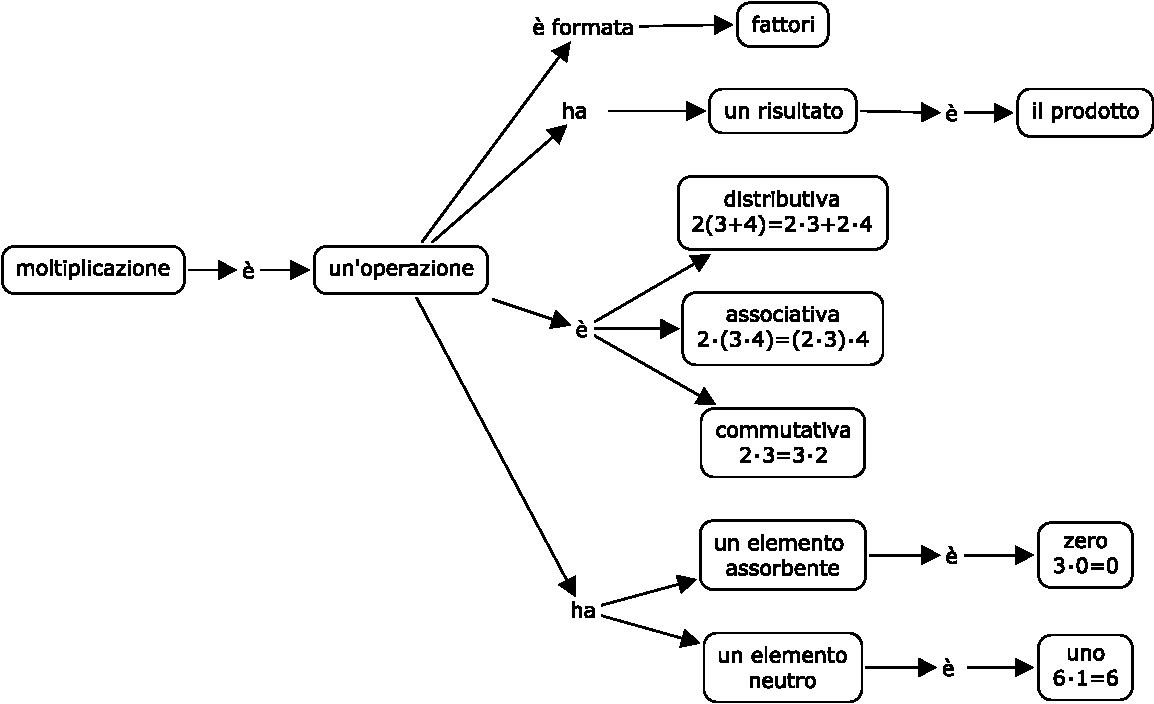
\includegraphics[scale=0.80]{Numerinaturali_prodotto-crop}
\section{Divisione}
\label{sec:Numerinatdiv}
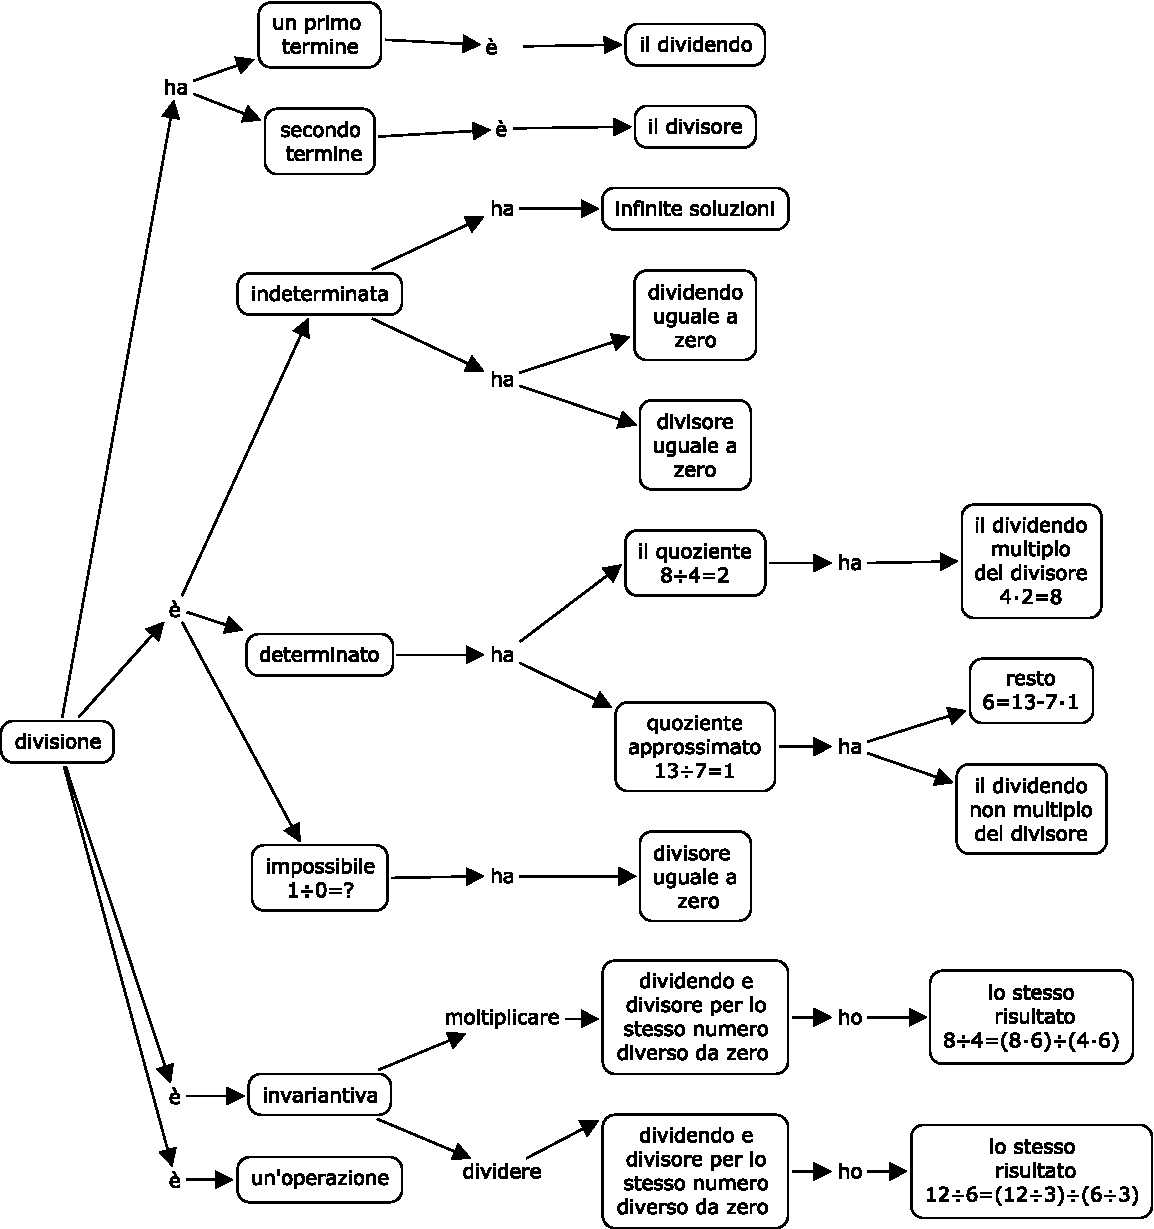
\includegraphics[scale=0.80]{Numerinaturali_divisione-crop}
\section{Potenza}
\label{sec:NumerinatPot}
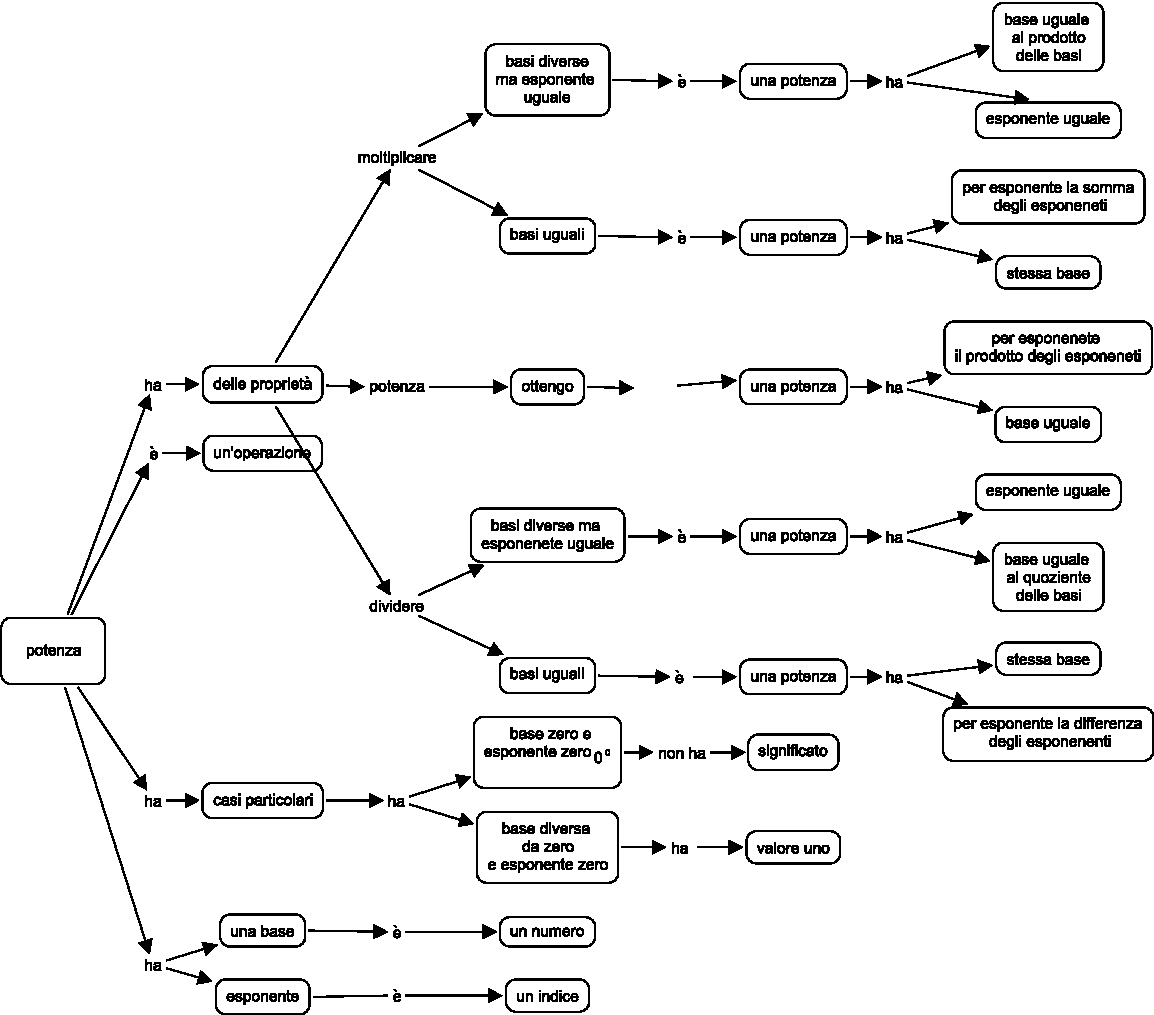
\includegraphics[scale=0.80]{Numerinaturali_potenza-crop}
\section{Numeri primi e composti}
\label{sec:Numeriprimiecomposti}
Una possibile classificazione dei numeri naturali è la seguente
\begin{center}
	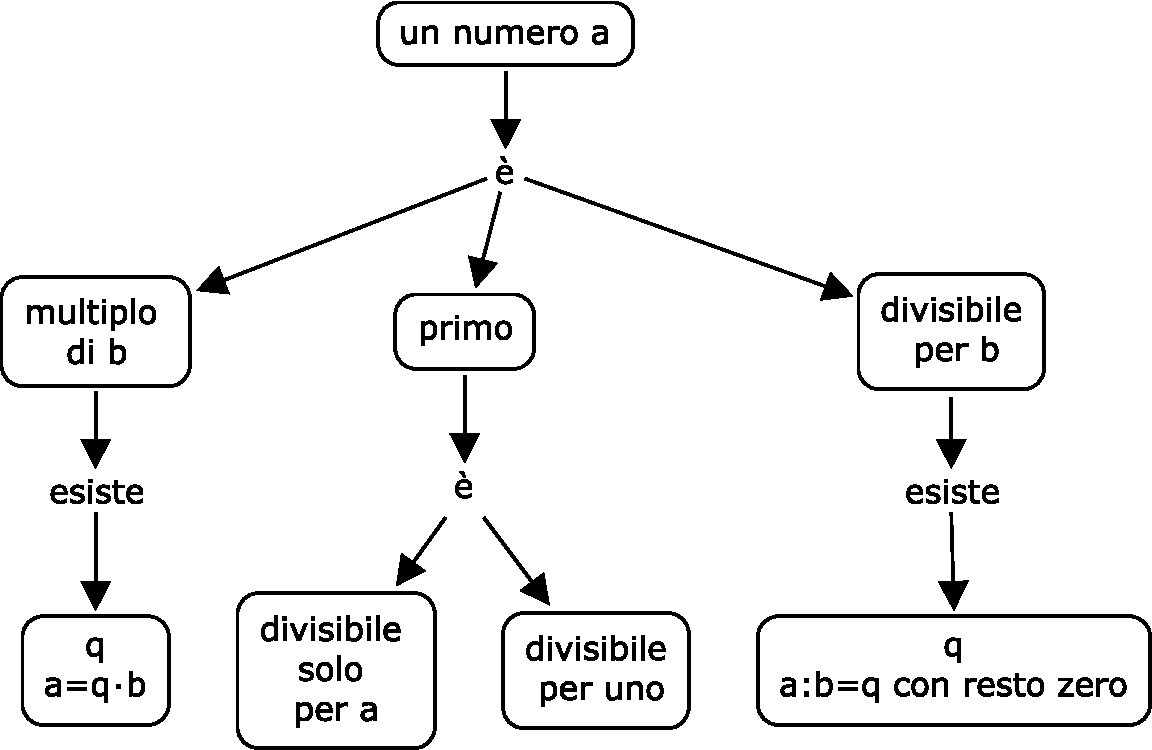
\includegraphics[scale=0.70]{NumeriNaturali_primi-crop}
\end{center}
Quindi, per esempio, dato che $18:2=9$ con resto zero avremo:
\begin{enumerate}
	\item 18 è multiplo di 2 secondo 9
	\item 18 è divisibile per 2
\end{enumerate}
\subsection{Scomposizione in fattori primi}
Per scomporre un numero naturale come prodotto di numeri primi  si può usare  l'algoritmo\nobs\vref{fig:numnatscposizionefattori}
	
\begin{figure}
\centering
\begin{tikzpicture}[auto, -stealth, thick]
% Definizione dei nodi e delle loro scatole
\tikzstyle{line} = [draw,->]
\node[ellipse,draw ]  (primo) {Inizio};
\node[rectangle,draw, text width=6cm,align=flush center, below of=primo, node distance=5em]  (secondo) {dividi il numero dato per
	il più piccolo primo che lo divide};
\node[diamond,draw, below of=secondo,node distance=10em]  (terzo) {il quoziente è uno?};
\node[ellipse, draw,below of=terzo,node distance=10em ] (quarto) {Fine};

% collegamento dei nodi
\begin{scope}[every path/.style=line]
\path  (primo) --  (secondo);
\path (secondo) edge  (terzo);
\path (terzo)  -- node  {SI} (quarto);
\path (terzo.west)  -|  node [near start] {NO} +(-7em,0) |- (secondo);
\end{scope}
\end{tikzpicture}
	\caption{Scomposizione in fattori primi}
	\label{fig:numnatscposizionefattori}
\end{figure}
	
Esempio 

\primedecomp{252}

quindi $252=2^2\cdot 3^2\cdot 7$

Esempio
\primedecomp{125}
$125=5^3$
	
\section{Massimo Comun Divisore}
\label{sec:macdNaturali}

Dati due o più numeri, il $\mcd$ è il numero\index{mcd} più grande che li divide tutti. Vi sono casi, in cui il $\mcd$ vale uno, perché uno è l'unico numero che li divide entrambi. Esempio di ciò sono il numero 8 e il numero nove, tranne l'uno non vi sono numeri naturali che li dividono entrambi. In questo caso si dice
 che i due numeri sono primi fra di loro.
 	
\begin{figure}
	\centering
\begin{tikzpicture}[node distance=8em,auto, -stealth, thick ,align=flush center,scale=0.4]
% Definizione dei nodi e delle loro scatole
\tikzstyle{line} = [draw,->]
\node[ellipse, draw,node distance=2em] (primo) {Inizio};
\node[rectangle,draw,below of=primo,text width=2cm](secondo) {Scomponi il numero in fattori primi};
\node[diamond,draw,below of=secondo,text width=2cm ]  (terzo) {I numeri dati sono finiti};
\node[rectangle,draw,below of=terzo,text width=2.2cm] (quarto) {Allineo le scomposizioni ottenute};
\node[diamond,draw,below of=quarto,text width=2cm]  (cinque) {Vi sono fattori in comune?};
\node[rectangle,draw,right of=cinque]  (sei) {mcd=1};
\node[rectangle,draw,below of=cinque,text width=2cm] (sette) {Prendo i fattori comuni con il minore esponenete};
\node[rectangle,draw,below of =sette,text width=2cm]  (otto) {mcd=prodotto dei fattori trovati};
\node[ellipse ,draw,below of=otto]  (nove) {Fine};
\begin{scope}[every path/.style=line]
\path  (primo) --  (secondo);
\path (secondo) edge  (terzo);
\path (terzo)  -- node  {SI} (quarto);
\path (terzo.west)  -|  node [near start]  {NO}+(-5em,0)  |-  (secondo);
\path(quarto)--(cinque);
\path (cinque.east)-- node [near start]{NO} (sei);
\path(cinque)--node[near start] {SI}(sette);
\path (sette)--(otto);
\path(otto)--(nove);
\end{scope}
\end{tikzpicture}
	\caption{Massimo Comun Divisore}
	\label{fig:numnatmcd}
\end{figure}

Esempio: per calcolare $\mcd(120,80,45)$ scompongo in fattori  primi i tre numeri come spiegato a\nobs\vref{fig:numnatscposizionefattori} e seguo lo schema\nobs\vref{fig:numnatmcd}     	
    \begin{tabular}{ccc}
    			\primedecomp{120}&\primedecomp{80}&\primedecomp{45}\\
    	\end{tabular}
    
    Allineo le scomposizioni
    
    \begin{tabular}{c}
    		$120=2^3\cdot 3\cdot5$\\
    	    $80=2^4\cdot 5$\\
    	    $45=3^2\cdot 5$
    \end{tabular}	
    
    I fattori comuni sono $2$ e $3$
    quindi $\mcd=2^3\cdot 3\cdot 5$
    \begin{figure}
    	\centering
    	\begin{tikzpicture}[auto, -stealth, thick, scale=0.5]
    	% Definizione dei nodi e delle loro scatole
    	\tikzstyle{line} = [draw,->]
    	\node[ellipse,draw] (zero) {Inizio};
    	\node[rectangle, draw,below of=zero, node distance=5em ]  (primo) {a,b};
    	\node[diamond,,draw,below of=primo,  node distance=5em]  (secondo) {b=0};
    	\node[rectangle,draw,right of= secondo,  node distance=10em]  (terzo) {mcd=a};
    	\node[rectangle,draw,below of= secondo,  node distance=5em]  (quarto) {a/b};
    	\node[diamond,,draw,below of=quarto,  node distance=5em]  (quinto) {resto=0};
    	\node[rectangle,draw,right of= quinto,  node distance=10em]  (sesto) {mcd=b};
    	\node[rectangle,draw,below of= quinto,  node distance=5em]  (settimo) {a=b b=r};
    	\node[ellipse,draw,below of= terzo,  node distance=5em]  (ottavo) {stop};
    	\node[ellipse,draw,below of=sesto,  node distance=5em]  (nono) {stop};
    	% collegamento dei nodi
    	\begin{scope}[every path/.style=line]
    	\path  (zero) edge  (primo);
    	\path  (primo) edge  (secondo);
    	%\path (secondo) edge  (terzo);
    	\path (secondo)  -- node  {SI} (terzo);
    	\path (secondo)  -- node  {NO} (quarto);
    	\path (quarto) edge  (quinto);
    	%\path (quinto) edge  (sesto);
    	\path (quinto)  -- node  {SI} (sesto);
    	\path (quinto)  -- node  {NO} (settimo);
    	\path (settimo.west)  -|  node [near start] {NO} +(-6em,0) |- (quarto);
    	\path (terzo) edge  (ottavo);
    	\path (sesto) edge  (nono);
    	\end{scope}
    	\end{tikzpicture}
    	\caption{Algoritmo di Euclide}
    	\label{fig:algoritmoEuclide}
    \end{figure}
   
   Un modo veloce per calcolare il $\mcd$ è l'algoritmo di Euclide\index{mcd!Euclide}. La figura\nobs\vref{fig:algoritmoEuclide} mostra la versione con divisione. Supponiamo di voler calcolare il $\mcd$ di $a=\num{27}$ e di $b=\num{15}$. Seguiamo lo schema, dividiamo $a$ con $b$ otteniamo un quoziente di 1 e un resto di $12$. Il resto non è $0$ per cui $a=\num{15}$ e di $b=\num{12}$ e ripetiamo. Dividiamo $a$ con $b$ otteniamo un quoziente di 1 e un resto di $3$. Il resto non è $0$ per cui $a=\num{15}$ e di $b=\num{3}$ e ripetiamo.  Dividiamo $a$ con $b$ otteniamo un quoziente di $5$ e un resto di $0$. Il resto è $0$ per cui $\mcd=\num{3}$    
   
   Supponiamo di voler calcolare il $\mcd$ fra \num{40} e \num{12}. Organizzo i calcoli come nella tabella\nobs\vref*{tab:euclidemcd1}. Inizio dividendo \num{40} per \num{12}. Ottengo come quoziente  \num{3} e per resto  \num{4}. La seconda riga ha per $a$ il precedente valore di $b$ e per $b$ il valore di $r$. Divido  \num{12} per \num{4}. Ottengo come quoziente  \num{3} e per resto  \num{0}. Essendo il resto uguale a zero, $\mcd(40;12)=4$
   \begin{table}
   	\centering
   	\begin{tabular}{SSSS}
   		\toprule
   		$a$&$b$&$a/b$&$r$\\
   		\midrule
   		40&12&3&4\\
   		12&4&3&0\\
   		\bottomrule
   	\end{tabular}
   	\caption[]{$\mcd$ \num{40} e \num{12}}
   	\label{tab:euclidemcd1}
   	\end{table} 
   	
   	Un esempio un po più lungo è nella tabella\nobs\vref*{tab:euclidemcd2}. In questo caso calcoliamo il $\mcd$ fra \num{85} e \num{26}. Dopo qualche passaggio otteniamo che il resto è zero quando $b=1$, quindi $\mcd(\num{85};\num{26})=1$. I numeri sono primi fra di loro. 
   	\begin{table}
   		\centering
   		\begin{tabular}{SSSS}
   			\toprule
   			$a$&$b$&$a/b$&$r$\\
   			\midrule
   			85&26&3&7\\
   			26&7&3&5\\
   			7&5&1&2\\
   			5&2&2&1\\
   			2&1&2&0\\
   			\bottomrule
   		\end{tabular}
   		\caption[]{$\mcd$ \num{85} e \num{26}}
   		\label{tab:euclidemcd2}
   	\end{table} 
    \section{Minimo comune multiplo}
        	\label{sec:mcmnumerinaturali}
     Il minimo comune multiplo fra due più o numeri è il più piccolo multiplo  in comune fra i numeri dati. 
    Esempio: per calcolare $\mcm(120,80,45)$ scompongo in fattori  primi i tre numeri come spiegato a\nobs\vref{fig:numnatscposizionefattori} e seguo lo schema\nobs\vref{fig:numnatmcm}     	
    	
    \begin{tabular}{ccc}
    		\primedecomp{120}&\primedecomp{80}&\primedecomp{45}\\
    	\end{tabular}
    	
    	Allineo le scomposizioni
    	
    	\begin{tabular}{c}
    		$120=2^3\cdot 3\cdot5$\\
    		$80=2^4\cdot 5$\\
    		$45=3^2\cdot 5$
    	\end{tabular}	
    	
    	quindi $\mcm=2^4\cdot 3^2\cdot 5$
    	
    	\begin{figure}
    		\centering
    		\begin{tikzpicture}[auto, -stealth, thick, scale=0.4]
    		% Definizione dei nodi e delle loro scatole
    		\tikzstyle{line} = [draw, -latex']
    		\node[ellipse, minimum height=4em, draw, very thick,inner xsep=3em] at (0,0) (primo) {Inizio
    		};
    		\node[rectangle,minimum height=4em,draw, very thick, text width=5cm,align=flush center] at (0,-4) (secondo) {Scomponi il numero in fattori primi};
    
    		\node[diamond,aspect=2,draw, very thick,inner xsep=3em, text width=2cm,align=flush center] at (0,-10
    		) (terzo) {I numeri dati sono finiti};
    		\node[rectangle,minimum height=4em,draw, very thick, text width=5cm,align=flush center] at (0,-17
    		) (quarto) {Allineo le scomposizioni ottenute};
    		\node[rectangle,minimum height=4em,draw, very thick, text width=5cm,align=flush center] at (0,-22)
    		(cinque) {Prendo i fattori comuni e non comuni con il maggiore esponente};
    		\node[rectangle,minimum height=4em,draw, very thick, text width=5cm,align=flush center] at (0,-27)
    		(sei) {mcm=prodotto dei fattori trovati};
    		
    		\node[ellipse ,minimum height=3em,draw, very thick,inner xsep=3em] at (0,-31) (sette) {Fine};
    			% collegamento dei nodi
    		\begin{scope}[every path/.style=line]
    		\path  (primo) --  (secondo);
    		\path (secondo) edge  (terzo);
    		\path (terzo)  -- node  {SI} (quarto);
    		\path (terzo.west)  -|  node [near start] {NO}+(-5em,0) |- (secondo);
    	
    		\path(quarto)--(cinque);
    		\path(cinque)--(sei);
    		\path(sei)--(sette);
    		
    		\end{scope}
    		\end{tikzpicture}
    			\caption{$\mcm$}
    			\label{fig:numnatmcm}
    		\end{figure}
  
	\chapter{Numeri razionali assoluti}
\label{cha:NumeriRazionaliAssoluti}
\minitoc
\mtcskip                                % put some skip here
\minilof                                % a minilof
\mtcskip                                % put some skip here
\minilot
\section{Frazione}
\label{sec:fraczioniNumRazASS}
Una frazione è il quoziente di una divisione. Alla frazione $\dfrac{a}{b}$ corrisponde la divisione $a\div b$ e viceversa.
\[
\text{Frazione}=
\dfrac{\text{Numeratore}}{\text{Denominatore}}
\]
Una frazione è\begin{itemize}
	\item Propria: il numeratore è minore del denominatore. Es. $\dfrac{2}{3}$ e $\dfrac{7}{8}$
	\item Impropria: il numeratore è maggiore del denominatore. Es. $\dfrac{3}{2}$ e $\dfrac{8}{7}$.
	
	Una frazione impropria può essere scritta come somma di un numero intero e di una frazione propria. 
	
	Esempio: $\dfrac{12}{5}=\dfrac{10}{5}+\dfrac{2}{5}=2+\dfrac{2}{5}$ 
	\item Apparente: il numeratore è un multiplo del denominatore. In questo caso la frazione coincide con un numero intero. Es. $\dfrac{8}{4}$ e $\dfrac{10}{5}$
\end{itemize}
\section{Numeri decimali}
\label{Numeri decimali}
\begin{tikzpicture}[very thick,node distance=5cm,text centered,minimum size=3cm,->=latex]
\node [circle, draw] (a) {Frazione};
\node [circle, draw] (b) [above right=of a] {Numero decimale};
\node [circle, draw] (c) [above left=of a]{Percentuale};
\draw [<->] (a) to (b);
\draw [<->] (b) to (c);
\draw [<->] (c) to (a);
\end{tikzpicture}
\subsection{Da frazione a numero decimale}
\begin{figure}
	\centering
	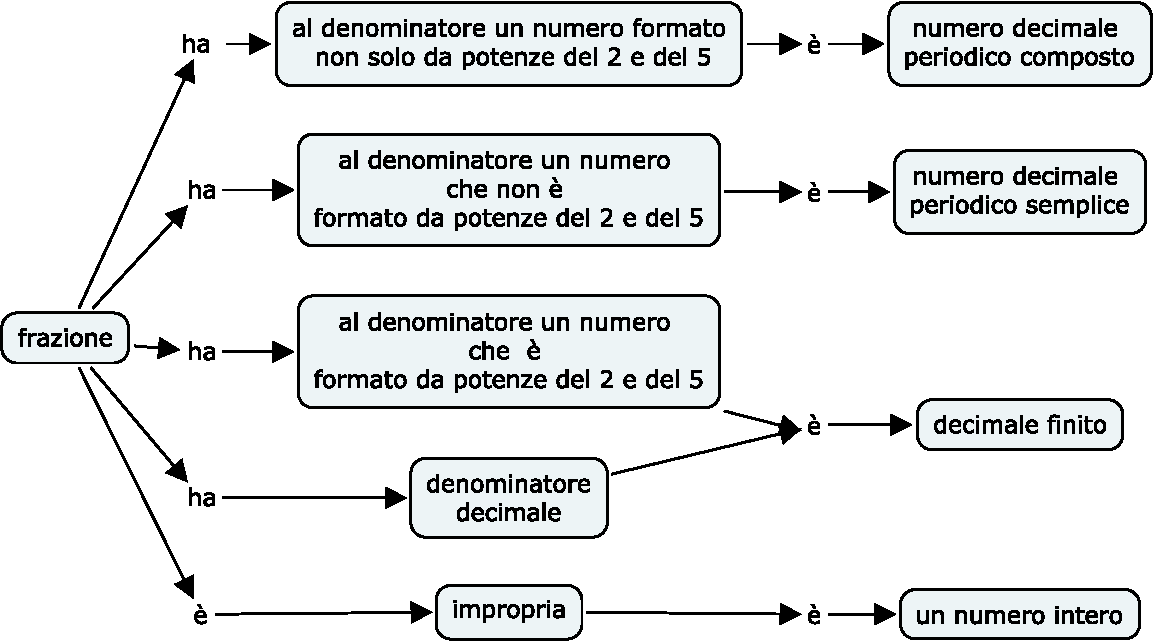
\includegraphics[scale=0.8]{da_frazione_a_numero_decimale-crop}
	\caption{Da frazione a decimale}
	\label{fig:DaFrazioniaDecimale}
\end{figure}
Una frazione è il quoziente di una divisione quindi ad una frazione è associata una divisione. Avremo molti casi fra loro diversi:
\begin{itemize}
	\item La frazione è una frazione apparente. In questo caso ad una frazione corrisponde un numero intero esempio: \[\dfrac{8}{4}=\num{2}\]
	\item La frazione ha per denominatore una potenza del dieci allora alla frazione corrisponde un numero decimale finito esempio:\[\dfrac{3}{10}=\num{0.3}\] 
	\item La frazione ha per denominatore un numero formato da potenze del \num{2} e del \num{5}. In questo caso è possibile trasformare la frazione in una frazione decimale. Esempio: \[\dfrac{3}{8}\] In questo casi si procede in questo modo\begin{enumerate}
		\item Si scompone il denominatore in numeri primi in questo caso $8=2^3$
		\item Si considera la seguente tabella 
		\begin{align*}
		\num{10}&=2\cdot 5\\
		\num{100}&=2^2\cdot 5^2\\
		\num{1000}&=2^3\cdot 5^3\\
		\num{10000}&=2^4\cdot 5^4\\
		\cdots&\cdots
		\end{align*}
		Da cui si vede che $2^3$ moltiplicato per $5^3$ da come risulto \num{1000}. Per cui, applicando al proprietà invariantiva che ci garantisce l'equivalenza delle frazioni abbiamo:\[\dfrac{3}{8}=\dfrac{3}{8}\cdot\dfrac{5^3}{5^3}=\dfrac{375}{1000}=\num{0,375}\] che è un decimale finito.
	\end{enumerate}
	Analogo esempio per \[\dfrac{7}{20}=\dfrac{7}{2^2\cdot 5}=\dfrac{7}{2^2\cdot 5}\cdot\dfrac{5}{5}=\dfrac{35}{100}=\num{0,35}\]
	\item La frazione ha per denominatore un numero non formato da potenze del \num{2} e del \num{5}. Il numero decimale ottenuto è un numero decimale periodico semplice, esempio:\[\dfrac{7}{9}=0{,}77777777\cdots=0{,}\overline{7}\]\[\dfrac{15}{11}=1{,}3636363636\cdots=1{,}\overline{36}\]
	\item La frazione ha per denominatore un numero anche da potenze del \num{2} e del \num{5}. Il numero decimale ottenuto è un numero decimale periodico misto esempio:\[\dfrac{15}{22}=0{,}68181818181818\cdots=0{,}68\overline{18}\]\[\dfrac{33}{14}=2{,}357142857142857\cdots=2{,}357\overline{142857}\]
\end{itemize}
Le parti di un numero decimale hanno un nome che è bene sapere %\[77.825=\overbrace{77}^{\text{parte intera}}.\underbrace{\overline{825}}_{\text{parte decimale}}\]
%\[2.357\overline{142857}=\overbrace{2}^{\text{parte intera}}.\underbrace{\underbrace{357}_{\text{antiperiodo}}\overbrace{\overline{142857}}^{\text{periodo}}}_{\text{parte decimale}} \]
\[\setlength{\tabcolsep}{1pt}
\begin{tabular}{r@{}cccccc}
&&&&\multicolumn{3}{c}{\tiny parte decimale}\\
\addlinespace[-.4ex]
\cmidrule(lr){5-7}
\addlinespace[-1ex]
&&\tiny parte intera&&\tiny antiperiodo&&\tiny periodo\\
\addlinespace[-.4ex]
\cmidrule{3-3}\cmidrule{5-5}\cmidrule{7-7}
\addlinespace[-.4ex]
$2{,}357\overline{142857}$&${}={}$&$2$&,&$357$&&$142857$
\end{tabular}
\]
\subsection{Da numero decimale a frazione}
Possiamo avere due alternative:
\begin{enumerate}
	\item Il numero decimale è un decimale finito. 
	
	Esempi: \numlist{2,3;34,567;0.007} 
	\[\begin{tabular}{ccc}
	$\num{2,3}=\dfrac{23}{10}$&$\num{34.567}=\dfrac{34567}{1000}$&$\num{0.007}=\dfrac{7}{1000}$
	\end{tabular}\]
	Quindi per trovare la frazione generatrice si mette a denominatore il numero senza la virgola e al denominatore una potenza del \num{10} con tanti zeri quanto è lunga la parte decimale.
	\item Il numero decimale è un numero decimale infinito periodico. 
	Esempi: 
	
	\begin{NodesList}
		\centering
		\begin{align*}
		\num{27,49}\overline{932}=\AddNode\\ %[.5cm] 
		=\dfrac{\num{2749932} -\phantom{2749}}{\phantom{99900}}=\AddNode\\[.5cm] %\AddNode[2]\\ 
		=\dfrac{\num{2747932}-\num{2747}}{\phantom{99900}}=\AddNode\\[.5cm]
		=\dfrac{\num{2747932}-\num{2747}}{\num{999}\phantom{00}}=\AddNode\\
		=\dfrac{\num{2747932}-\num{2747}}{\num{99900}}=\AddNode\\
		=\dfrac{\num{2747185}}{\num{99900}}\AddNode
		\end{align*}
		\LinkNodes[margin=3cm]{\begin{minipage}[h]{3.5cm}
				Prendo tutto il numero senza la virgola
			\end{minipage}}
			\LinkNodes[margin=3cm]{\begin{minipage}[h]{3.5cm}
					Sottraggo il numero escluso il periodo
				\end{minipage}}%
				\LinkNodes[margin=3cm]{\begin{minipage}[h]{3.5cm}
						Il periodo è lungo tre divido per $999$
					\end{minipage}}%
					\LinkNodes[margin=3cm]{\begin{minipage}[h]{3.5cm}
							L'antiperiodo è lungo $2$ aggiungo quindi due zeri 
						\end{minipage}}%
						\LinkNodes[margin=3cm]{\begin{minipage}[h]{3.5cm}
								Ottengo
							\end{minipage}}%
						\end{NodesList}
						
\begin{NodesList}
		\centering
		\begin{align*}
		\num{7,4}\overline{25}=\AddNode\\[.5cm] 
		=\dfrac{\num{7425}-\phantom{74}}{\phantom{990}}=\AddNode\\ %[.5cm] %\AddNode[2]\\ 
		=\dfrac{\num{7425}-\num{74}}{\phantom{990}}=\AddNode\\[.5cm]
		=\dfrac{\num{7425}-\num{74}}{\num{99}\phantom{0}}=\AddNode\\
		=\dfrac{\num{7425}-\num{74}}{\num{990}}=\AddNode\\
		=\dfrac{\num{7351}}{\num{990}}\AddNode
		\end{align*}
		\LinkNodes[margin=3cm]{\begin{minipage}[h]{3.5cm}
				Prendo tutto il numero senza la virgola
			\end{minipage}}
			%\LinkNodes{Sposto $2x$ a sinistra e cambio di segno}%
			\LinkNodes[margin=3cm]{\begin{minipage}[h]{3.5cm}
					Sottraggo il numero escluso il periodo
				\end{minipage}}%
				\LinkNodes[margin=3cm]{\begin{minipage}[h]{3.5cm}
						il periodo è lungo due quindi divido per $99$
					\end{minipage}}%
					\LinkNodes[margin=3cm]{\begin{minipage}[h]{3.5cm}
							L'antiperiodo è lungo uno quindi aggiungo uno zero 
						\end{minipage}}%
						\LinkNodes[margin=3cm]{\begin{minipage}[h]{3.5cm}
								Ottengo
							\end{minipage}}%
						\end{NodesList}
	
	\begin{NodesList}
		\centering
		\begin{align*}
		\num{35},\overline{5}=\AddNode\\[.5cm] 
		=\dfrac{\num{355} -\phantom{35}}{\phantom{9}}=\AddNode\\[.5cm] %\AddNode[2]\\ 
		=\dfrac{\num{355}-\num{35}}{\phantom{9}}=\AddNode\\[.5cm]
		=\dfrac{\num{355}-\num{35}}{\num{9}}=\AddNode\\
		%	=\dfrac{\num{2747932}-\num{2747}}{\num{99900}}=\AddNode\\
		=\dfrac{\num{320}}{\num{9}}\AddNode
		\end{align*}
		\LinkNodes[margin=3cm]{\begin{minipage}[h]{3.5cm}
				Prendo tutto il numero senza la virgola
			\end{minipage}}
			\LinkNodes[margin=3cm]{\begin{minipage}[h]{3.5cm}
					Sottraggo il numero escluso il periodo
				\end{minipage}}%
				\LinkNodes[margin=3cm]{\begin{minipage}[h]{3.5cm}
						Il periodo è lungo uno divido per $9$
					\end{minipage}}%
					%	\LinkNodes{\begin{minipage}[h]{3.5cm}
					%	L'antiperiodo è lungo $2$ aggiungo quindi due zeri 
					%		\end{minipage}}%
					\LinkNodes[margin=3cm]{\begin{minipage}[h]{3.5cm}
							Ottengo
						\end{minipage}}%
	\end{NodesList}
	
	\begin{NodesList}
		\centering
		\begin{align*}
		\num{0},\overline{25}=\AddNode\\[.5cm] 
		=\dfrac{\num{25} -\phantom{0}}{\phantom{99}}=\AddNode\\[.5cm] %\AddNode[2]\\ 
		=\dfrac{\num{25}-\num{0}}{\phantom{99}}=\AddNode\\[.5cm]
		=\dfrac{\num{25}-\num{0}}{\num{99}}=\AddNode\\
		%	=\dfrac{\num{2747932}-\num{2747}}{\num{99900}}=\AddNode\\
		=\dfrac{\num{25}}{\num{99}}\AddNode
		\end{align*}
		\LinkNodes[margin=3cm]{\begin{minipage}[h]{3.5cm}
				Prendo tutto il numero senza la virgola
			\end{minipage}}
			\LinkNodes[margin=3cm]{\begin{minipage}[h]{3.5cm}
					Sottraggo il numero escluso il periodo
				\end{minipage}}%
				\LinkNodes[margin=3cm]{\begin{minipage}[h]{3.5cm}
						Il periodo è lungo due divido per $99$
					\end{minipage}}%
					%	\LinkNodes{\begin{minipage}[h]{3.5cm}
					%	L'antiperiodo è lungo $2$ aggiungo quindi due zeri 
					%		\end{minipage}}%
					\LinkNodes[margin=3cm]{\begin{minipage}[h]{3.5cm}
							Ottengo
						\end{minipage}}%
					\end{NodesList}
					
\begin{NodesList}
	\centering
	\begin{align*}
	\num{0},3\overline{47}=\AddNode\\[.5cm] 
	=\dfrac{\num{347} -\phantom{3}}{\phantom{99}}=\AddNode\\[.5cm] %\AddNode[2]\\ 
	=\dfrac{\num{347}-\num{3}}{\phantom{99}}=\AddNode\\[.5cm]
	=\dfrac{\num{347}-\num{3}}{\num{99}\phantom{0}}=\AddNode\\
	=\dfrac{\num{347}-\num{3}}{\num{990}}=\AddNode\\
	=\dfrac{\num{344}}{\num{990}}\AddNode
	\end{align*}
	\LinkNodes[margin=3cm]{\begin{minipage}[h]{3.5cm}
			Prendo tutto il numero senza la virgola
		\end{minipage}}
		\LinkNodes[margin=3cm]{\begin{minipage}[h]{3.5cm}
				Sottraggo il numero escluso il periodo
			\end{minipage}}%
			\LinkNodes[margin=3cm]{\begin{minipage}[h]{3.5cm}
					Il periodo è lungo due divido per $99$
				\end{minipage}}%
				\LinkNodes[margin=3cm]{\begin{minipage}[h]{3.5cm}
						L'antiperiodo è lungo $1$ aggiungo quindi uno zero 
					\end{minipage}}%
					\LinkNodes[margin=3cm]{\begin{minipage}[h]{3.5cm}
							Ottengo
						\end{minipage}}%
	\end{NodesList}
	Per trovare la frazione generatrice bisogna togliere la virgola e sottrarre al numero con la parte periodica compresa il numero senza la parte periodica e dividere per un numero composto da tanti nove per quanto è lungo il periodo e tanti zero per quanto è lungo l'antiperiodo. Il perché di questa regola può essere spiegato con questi esempi:
	\begin{enumerate}
		\item Per trovare la funzione generatrice di $x=7{,}2\overline{4}$ si procede in questo modo
		\begin{align*}
		%x=&7{,}2\overline{4}\\
		100x &=724{,}\overline{4}\\
		10x &=72{,}\overline{4}\\
		100x-10x&=724{,}\overline{4}-72{,}\overline{4}=652\\
		90x&=652\\
		x&=\dfrac{652}{90}
		\end{align*}
		\item Per trovare la funzione generatrice di $x=1{,}\overline{2}$ si procede in questo modo
		\begin{align*}
		%	x=&1{,}\overline{2}\\
		10x &=12{,}\overline{2}\\
		x &=1{,}\overline{2}\\
		10x-x&=12{,}\overline{2}-1{,}\overline{2}=11\\
		9x&=11\\
		x&=\dfrac{11}{9}
		\end{align*}
		\item Per trovare la funzione generatrice di $x=1{,}\overline{22}$ si procede in questo modo
		\begin{align*}
		%	x=&1{,}\overline{22}\\
		100x &=122{,}\overline{22}\\
		x &=1{,}\overline{22}\\
		100x-x&=122{,}\overline{22}-1{,}\overline{22}=121\\
		99x&=121\\
		x&=\dfrac{121}{99}
		\end{align*}
	\end{enumerate}
	
\end{enumerate}
Un piccolo gioco 
\[0{,}\overline{9}=1\]
\subsection{Da numero percentuale a decimale}
Per trasformare un numero percentuale in numero decimale basta dividere il numero per cento. 

Esempi:\[10\%= 10:100=0,1 \] \[82,5\%= 82,5:100=0,825 \]
\subsection{Da numero decimale a percentuale}
Per trasformare un numero decimale in percentuale basta moltiplicare il numero per $\dfrac{100}{100}$

Esempio \[\num{4,5}=4,5\cdot\dfrac{100}{100}=\dfrac{450}{100}=450\%\]
\[\num{0,58}=0{,}58\cdot\dfrac{100}{100}=\dfrac{58}{100}=58\%\]
\subsection{Da percentuale a frazione}
Per trasformare una percentuale in una frazione basta ricordare che una percentuale è una divisione per cento.
Esempio
\[20\%=\dfrac{20}{100} \]
\subsection{Da frazione a percentuale}
La trasformazione è in due tempi 
\begin{enumerate}
	\item Trasformo la frazione in un numero decimale
	\item Trasformo il numero decimale in percentuale
\end{enumerate}
Esempio 
\[\dfrac{75}{4}=18,75=18,75\cdot\dfrac{100}{100}=1875\% \]

\section{Frazioni equivalenti}
\label{sec:FrazioniEquivalentiNumRazzASS}
Due frazioni sono equivalenti quando rappresentano lo stesso quoziente. Esempio  $\dfrac{3}{4}$ e $\dfrac{6}{8}$ sono equivalenti e  si scrive \[\dfrac{2}{3} \equiv\dfrac{6}{8}\]

Se due frazioni sono equivalenti vale il cosiddetto prodotto in croce e viceversa, cioè:
\begin{center}
\prodcroce{A}{B}{C}{D}
\end{center}
Esempio 
%\begin{document}
\begin{center}
\prodcroce{3}{4}{6}{8}
\end{center}
quindi le due frazioni sono equivalenti
\section{Proprietà  invariantiva}
\label{sec:propInvariantivaNumASS}

Moltiplicando o dividendo per un numero diverso da zero il numeratore e il denominatore di una frazione si ottiene una frazione equivalente 
infatti $\dfrac{a}{b}=\dfrac{ac}{bc}$
\begin{center}
 \prodcroce{a}{b}{ac}{bc}
\end{center}

Esempio

\[\dfrac{3}{4}=\dfrac{3\cdot 8}{4\cdot 8}=\dfrac{24}{32}\]   le due frazioni sono equivalenti infatti: 

\[\prodcroce{3}{4}{24}{32}\]

Esempio:

\[\dfrac{6}{8}=\dfrac{6:2}{8:2}=\dfrac{3}{4}\]   le due frazioni sono equivalenti infatti: 

\[\prodcroce{6}{8}{3}{4}\]
\section{Semplificare una frazione}
\label{sec:sempunaFrazASS}
Semplificare una frazione significa dividere il numeratore e il denominatore per il loro Massimo Comune Divisore (MCD). Per la proprietà invariantiva la frazione ottenuta è equivalente a quella data.
La procedura è quindi la seguente 

Data la frazione $\dfrac{a}{b}$

\begin{enumerate}
	\item Calcolo il $\mcd(a,b)$
	\item Divido il numeratore e il denominatore per  $\mcd(a,b)$
\end{enumerate}

Esempio 

Semplificare la frazione $\dfrac{84}{48}$  
\begin{enumerate}
	\item Inizio con  trovare il $\mcd(84,48)$ li scompongo in fattori primi e ottengo
	
	\begin{center}
	\begin{tabular}{cc}
		\primedecomp{84}&\primedecomp{48}\\
		$48 =2^4\cdot  3$&	$84=2^2\cdot 3\cdot 7$
	\end{tabular}
	\end{center}
	quindi $\mcd(84,48)=2^2\cdot 3=12$
	\item 	Divido numeratore e denominatore per 12 e ottengo $\dfrac{7}{4}$
\end{enumerate}
	Vi è un altro metodo per semplificare una frazione: Dividere se possibile numeratore e denominatore per uno stesso numero e continuare finché ciò è possibile come nell'esempio successivo.
	
	\begin{center}
	\begin{tikzpicture}[thick]
	\node at (0,0) {$\displaystyle \dfrac{84}{48}$};
	\node at (0.5,0.5) {$\displaystyle 42$};
	\node at (0.5,-0.5) {24};
	\node at (1,0.6){21};
	\node at (1,-0.6){12};
	\node at (1.4,0.7){7};
	\node at (1.4,-0.7){4};
	\end{tikzpicture}
	\end{center}
	%$\dfrac{\cancel{84}}{\cancel{48}}\rightarrow\dfrac{\cancel{42}}{\cancel{24}}\rightarrow\dfrac{\cancel{21}}{\cancel{12}}\rightarrow\dfrac{7}{4} $
	\section{Riduzione allo stesso denominatore}
	\label{sec:RiduzionestessoindiceFrazzASS}
	La proprietà invariantiva permette di trasformare due frazioni a denominatore diverso in due frazioni che hanno lo stesso denominatore.
	Il procedimento è il seguente 
	\begin{enumerate}
		\item Date le frazioni $\dfrac{5}{21}$ e $\dfrac{7}{12}$
		\item Scompongo i denominatori in fattori primi cioè:
		
		\begin{center}
			\begin{tabular}{cc}
				\primedecomp{21}&\primedecomp{12}\\
				$21=3\cdot 7$& $12=3\cdot 2^4$
			\end{tabular}
		\end{center}
	    \item Calcolo il $\mcm$ che in questo caso è $\mcm(21,12)=2^2\cdot 3\cdot 7=84$ 		
		\item Scrivo due frazioni con denominatore 84 cioè $\dfrac{}{84}$ e $\dfrac{}{84}$
		\item Applico la proprietà invariantiva al numeratore e scrivo $\dfrac{84:21\cdot 5}{84}$ e $\dfrac{84:12\cdot 7}{84}$
		\item Otteniamo $\dfrac{20}{84}$ e $\dfrac{49}{84}$
	\end{enumerate}
	\subsection{Confronto fra frazioni}
	Per confrontare due frazioni le riduco allo stesso denominatore è maggiore la frazione con denominatore maggiore.
	
	Esempio Ordinare in modo decrescente le seguenti frazioni
	\begin{align*}
		&\dfrac{1}{2}&\dfrac{1}{3}&&\dfrac{3}{5}&&\dfrac{3}{8}\\
		\text{Calcolo il mcm}\\
		&\dfrac{}{120}&\dfrac{}{120}&&\dfrac{}{120}&&\dfrac{}{120}\\
		\text{Riduco allo stesso denominatore}\\
		&\dfrac{60}{120}&\dfrac{40}{120}&&\dfrac{72}{120}&&\dfrac{45}{120}\\
	\end{align*}

		La frazione che ha il numeratore più grande è $\dfrac{72}{120}$ che corrisponde a $\dfrac{3}{5}$ questa è la frazione più grande. A questa
		segue $\dfrac{3}{8}$ perché corrisponde a $\dfrac{45}{120}$ e così di seguito $\dfrac{1}{2}$ ed infine $\dfrac{1}{3}$.
%\mediapriorita{Aggiungere esempi}
	\section{Operazioni}
	\label{sec:OperazioniASS}
	\subsection{Somma e sottrazione}
	\label{ssec:SommaesottrazioniASS}
	Nel sommare due frazioni possiamo avere due casi 
	\begin{enumerate}
		\item Denominatori uguali
		
		La somma/differenza due frazioni che hanno lo stesso denominatore è una frazione che ha lo stesso denominatore e per numeratore la somma/differenza dei numeratori. 
		
		Esempio: \[\dfrac{2}{3}+\dfrac{8}{3}=\dfrac{10}{3}\] Esempio \[\dfrac{12}{5}-\dfrac{8}{5}=\dfrac{4}{5}\]
		\item Denominatori diversi
		
		Riduco le due frazioni allo stesso denominatore come in\nobs\vref{sec:RiduzionestessoindiceFrazzASS} e quindi sommo.
		
		Esempio:\begin{align*}
		&\dfrac{2}{3}+\dfrac{7}{5}\\
		&\text{Calcolo}\\
		&\mcd(3,5)=15\\
		&\dfrac{15:3\cdot 2+15:5\cdot 7}{15}\\
		&\dfrac{10+21}{15}\\
		&\dfrac{21}{15}
		\end{align*}
	\end{enumerate}
	\begin{table}
		\centering
		\begin{tikzpicture}[auto, -stealth, thick, scale=0.5]
		% Definizione dei nodi e delle loro scatole
		\tikzstyle{line} = [draw, -latex']
		\node[ellipse, minimum height=4em, draw, very thick,inner xsep=3em] at (0,0) (primo) {Inizio};
		\node[rectangle,minimum height=4em,draw, very thick, text width=5cm,align=flush center] at (0,-5) (secondo) {Calcola mcm fra i denominatori};
		\node[rectangle,minimum height=4em,draw, very thick, text width=5cm,align=flush center] at (0,-11
		) (terzo) {Dividi il mcm per denominatore e moltiplico il risultato per il numeratore};
		\node[diamond,aspect=2,draw, very thick,inner xsep=3em, text width=2cm,align=flush center] at (0,-18) (quarto){ le frazioni sono finite?};
		\node[rectangle,minimum height=4em,draw, very thick, text width=5cm,align=flush center] at (0,-25) (quinto) {Somma i valori trovati};  		
		
		\node[ellipse ,minimum height=4em,draw, very thick,inner xsep=3em] at (0,-29) (sesto) {Fine};
		% collegamento dei nodi
		\begin{scope}[every path/.style=line]
		\path  (primo) --  (secondo);
		\path (secondo) edge  (terzo);
		\path (terzo)--(quarto);
		\path (quarto)  -- node  {SI} (quinto);
		\path (quarto.west)  -|  node [near start] {NO}+(-5em,0) |- (terzo);
		\path(quarto)--(quinto);
		\path(quinto)--(sesto);
		\end{scope}
		\end{tikzpicture}
		\caption{Somma di frazioni}
		\label{tab:sommadifrazioniASS}
	\end{table}
	\subsection{Moltiplicazione}
	\label{sec:MoltiplicazioneASS}
	Nel moltiplicare  due frazioni possiamo avere due casi 
	\begin{enumerate}
		\item frazione con frazione
		
		Esempio \begin{center}
					\begin{tikzpicture}[thick]
					\def\x{2.8mm}
					\def\h{2.4mm}
					\def\dist{10mm}%1cm
					\node at (0,0) {$\displaystyle \dfrac{21}{4}$};
					\node at (\dist,0) {$\displaystyle \dfrac{3}{5}$};
					\node at (\dist/2,0) {$\cdot$};
					\node  at (-\dist,0) {$\displaystyle \dfrac{21}{4}\cdot\displaystyle \dfrac{3}{5}= $};
					\draw[-stealth] (\x, -\h)--(\dist-\x,-\h);
					\draw[-stealth] (\x,\h)--(\dist -\x, \h);
					\node at (2.2*\dist,0) {$=\displaystyle \dfrac{21\cdot 3}{4\cdot 5}=\displaystyle \dfrac{63}{20}$};
					% \draw[-stealth] (-\x,\h)--(-\x, -\h);
					%   \draw[-stealth] (\dist+\x,\h)--(\dist+\x, -\h);
					\end{tikzpicture}%
		\end{center}
		
		quindi nella moltiplicazione fra due frazioni si  moltiplicano numeratore con numeratore e denominatore con denominatore.
		\item frazione con numero
	   
	   Esempio
	   
	   \begin{center}
	 \begin{tikzpicture}[thick]
	 \def\x{2.8mm}
	 \def\h{2.4mm}
	 \def\dist{10mm}%1cm
	 \node  at (-\dist,0) {$\displaystyle \dfrac{5}{4}\cdot 7 = $};
	 \node at (0,0) {$\displaystyle \dfrac{5}{4}$};
	 \node at (\dist,0) {$\displaystyle \dfrac{7}{1}$};
	 \node at (\dist/2,0) {$\cdot$};
	 
	 %	\draw[-stealth] (\x, -\h)--(\dist-\x,-\h);
	 \draw[-stealth] (\x,\h)--(\dist -\x, \h);
	 \node at (2.2*\dist,0) {$=\displaystyle \dfrac{5\cdot 7}{4}=\displaystyle \dfrac{35}{4}$};
	 % \draw[-stealth] (-\x,\h)--(-\x, -\h);
	 %   \draw[-stealth] (\dist+\x,\h)--(\dist+\x, -\h);
	 \end{tikzpicture}%
	   \end{center}
	   quindi nella moltiplicazione fra una frazione e un numero si moltiplica il numero con il numeratore e il denominatore resta uguale.
	\end{enumerate}
	\subsection{Semplificazioni e moltiplicazioni}
	Semplificare una frazione è possibile quando numeratore e denominatore sono divisibili per lo stesso numero. La semplificazione avviene quindi in verticale come per esempio:
	\begin{center}
		\begin{tikzpicture}[thick]
		\def\x{2.8mm}
		\def\h{2.4mm}
		\node at (0,0) {$\displaystyle \dfrac{4}{16}$};
		\node at (\x+15,0) {$\displaystyle= \dfrac{1}{4}$};
		\draw[-stealth] (-\x,\h)--(-\x, -\h);
		\draw[-stealth] (\x,\h)--(\x, -\h);
		\end{tikzpicture}%
	\end{center}
	
	Con la moltiplicazione è possibile anche la cosiddetta semplificazione in croce come per esempio: 
	         \begin{center}
	         	\begin{tikzpicture}[thick]
	         	\def\x{2.8mm}
	         	\def\h{2.4mm}
	         	\def\dist{12mm}%1cm
	         	\node at (0,0) {$\displaystyle \dfrac{5}{27}$};
	         	\node  at(-0.5,0.5) {1};
	         	\node  at(-0.5,-0.5) {3};
	         	\node at (\dist,0) {$\displaystyle \dfrac{9}{20}$};
	         	\node at (2*\dist+\x,0) {$\displaystyle =\dfrac{1\cdot 1}{3\cdot 4}=\dfrac{1}{12}$};
	         	\node at (\dist+10,0.5){1};
	         	\node at (\dist+10,-0.5){4};
	         	\draw[-stealth] (\x, \h)--(\dist-\x,-\h);
	         	\draw[-stealth] (\x,-\h)--(\dist -\x, \h);
	         	%\draw[-stealth] (-\x,\h)--(-\x, -\h);
	         	%\draw[-stealth] (\dist+\x,\h)--(\dist+\x, -\h);
	         	\end{tikzpicture}%
	         \end{center}	
	
	
	In questo caso è possibile semplificare il denominatore della prima frazione con il numeratore della seconda e il numeratore della prima con il denominatore della seconda.

\subsection{Divisione fra frazioni}

Prima di parlare di divisioni fra frazioni occorre parlare di reciproci. Due numeri sono reciproci se il loro prodotto è uno. Quindi per le frazioni avremo per esempio:\[\dfrac{2}{5}\cdot\dfrac{5}{2}=1\]In questo caso si dice che $\dfrac{2}{5}$ e $\dfrac{5}{2}$ sono frazioni fra loro reciproche.
Per un numero intero avremo per esempio\[2\cdot\dfrac{1}{2}=1\]

In pratica  avremo che per trovare il reciproco di un numero avremo due casi
\begin{enumerate}
	\item Il numero è una frazione. In questo caso basta scrivere una frazione con numeratore e denominatore scambiato fra loro.
	\item Il numero è un numero intero. In questo caso basta scrivere una frazione che ha per numeratore uno e per denominatore il numero di partenza 
\end{enumerate}

Per dividere due frazioni bisogna trasformare la divisione nel prodotto della prima per il reciproco della seconda. Esempio

\[\dfrac{7}{4}:\dfrac{4}{5}=\dfrac{7}{4}\cdot\dfrac{5}{4}=\dfrac{7\cdot 5}{5\cdot 4}\]



	\chapter{Le proporzioni}
\label{sec:LeProporzioni}
\minitoc%
\section{Proporzioni semplici}
\label{sec:ProporzioniSemplici}


Una proporzione è un'uguaglianza fra frazioni
\[\dfrac{a}{b}=\dfrac{c}{d}\]
\[medi\index{Proporzione!medi}\]
\[{\underbrace{a:\overbrace{b=c}:d}}\]
\[estremi\index{Proporzione!estremi}\]
\[a,b,c,d\in N\]

Una proporzione con i medi\index{Proporzione!medi} uguali si dice continua\index{Proporzione!continua}

\section{Proprietà delle proporzioni}
\label{sec:ProprietaDelleProporzioni}
\subsection{Propriet\'{a} fondamentale delle proporzioni}\label{prop:fond}
\begin{enumerate}
	\item In una proporzione il prodotto dei medi\index{Proporzione!medi} è uguale al prodotto degli estremi\index{Proporzione!estremi} \[a\cdot d= b\cdot c\]
	\item In una proporzione qualunque un medio incognito è uguale al prodotto degli estremi\index{Proporzione!estremi} fratto l'altro medio. 
	\begin{align*}
	a:x=c:d&\\
	x=\dfrac{a\cdot d}{c}&
	\end{align*}
	\item In una proporzione qualunque un estremo incognito è uguale al prodotto degli medi\index{Proporzione!medi} fratto l'altro medio. 
	\begin{align*}
	x:b=c:d&\\
	x=\dfrac{b\cdot c}{d}&
	\end{align*}
	\item Il medio proporzionale fra due numeri dati à uguale alla radice quadrata del  prodotto degli estremi.
		\begin{align*}
		a:x=x:d&\\
		x=\sqrt{a\cdot d}&
		\end{align*}
	\item In una proporzione la somma dei primi due termini sta al primo (secondo) come dei due restanti termini sta al terzo (quarto)\footnote{dimostriamo la prima uguaglianza:
		\begin{gather*}
		\dfrac{a}{b}=\dfrac{c}{d}\\
		\dfrac{a}{b}+1=\dfrac{c}{d}+1\\
		\dfrac{a+b}{b}=\dfrac{c+d}{d}
		\end{gather*}
		
		dimostriamo la seconda uguaglianza
		\begin{gather*}
		\dfrac{b}{a}=\dfrac{d}{c}\\
		\dfrac{b}{a}+1=\dfrac{d}{c}+1\\
		\dfrac{a+b}{a}=\dfrac{c+d}{c}
		\end{gather*}}
	\[(a+b):b = (c+d):d\]
	\[(a+b):a = (c+d):c\]
	\item In una proporzione la differenza fra il maggiore e il minore dei primi due termini sta al primo (secondo) come la differenza fra il maggiore e il minore dei due restanti termini sta al terzo (quarto)
	\[(a-b):a = (c-d):c\]
	\[(a-b):b = (c-d):d\]
	\item Una proporzione \'{e} ancora una proporzione scambiando fra loro i medi\index{Proporzione!medi} (o gli estremi\index{Proporzione!estremi})
	\item In una proporzione la somma degli antecedenti\index{Proporzione!antecedenti} sta alla somma dei conseguenti\index{Proporzione!conseguenti} come un antecedente sta al suo conseguente\footnote{\begin{gather*}
		\dfrac{c}{a}=\dfrac{d}{b}
		\\1+\dfrac{c}{a}=1+\dfrac{d}{b}
		\\ \dfrac{a+c}{a}=\dfrac{b+d}{b}
		\\ (a+c):a= (b+d):b
		\end{gather*}
		\[(a+c):(b+d)=a:b\]}.
	\[(a+c):(b+d)=a:b\]
	\item In una proporzione, la differenza tra il maggiore e il minore degli antecedenti,\index{Proporzione!antecedenti} sta alla differenza tra il maggiore e il minore dei conseguenti,\index{Proporzione!conseguenti} come un antecedente sta al suo conseguente.
	\[(a-c):(b-d)=a:b\]
\end{enumerate}
\section{Serie di rapporti uguali}
\label{sec:serieDiRapportiUguali}

Una serie di rapporti\index{Rapporti uguali!rapporti} uguali è l'uguaglianza fra tre o più frazioni\label{sec:sRaUguali}

\[
\dfrac{a_{1}}{b_{1}}=\dfrac{a_{2}}{b_{2}}=\cdots=\dfrac{a_{n}}{b_{n}}\qquad n\geq3\]
[Comporre generalizzata]\index{Rapporti uguali!comporre generalizzata}

In una serie di rapporti uguali la somma degli antecedenti sta alla somma dei conseguenti, come un antecedente sta al proprio conseguente\footnote{Dalla definizione\nobs\vref{sec:sRaUguali}
	\begin{gather*}
	\dfrac{a_{2}}{a_{1}}=\dfrac{b_{2}}{b_{1}}\\
	\dfrac{a_{3}}{a_{1}}=\dfrac{b_{3}}{b_{1}}
	\\
	\ldots%
	\\
	\dfrac{a_{n}}{a_{1}}=\dfrac{b_{n}}{b_{1}}
	\end{gather*}
	
	sommando membro a membro ottengo
	\[\dfrac{a_{2}}{a_{1}}+\dfrac{a_{3}}{a_{1}}+\cdots+\dfrac{a_{n}}{a_{1}}=\dfrac{b_{2}}{b_{1}}+\dfrac{b_{3}}{b_{1}}+\cdots+\dfrac{b_{n}}{b_{1}}\]
	da cui
	\[1+\dfrac{a_{2}}{a_{1}}+\dfrac{a_{3}}{a_{1}}+\cdots+\dfrac{a_{n}}{a_{1}}=\dfrac{b_{2}}{b_{1}}+\dfrac{b_{3}}{b_{1}}+\cdots+\dfrac{b_{n}}{b_{1}}+1\]
	da cui 
	\[\dfrac{a_{1}+a_{2}+\cdots+a_{n}}{a_{1}}=\dfrac{b_{1}+b_{1}+\cdots+b_{n}}{b_{1}}\]
	da cui la prima relazione.
	
	Procedendo in maniera analoga otteniamo il resto.}
\begin{gather*}
	(a_{1}+a_{2}+\ldots+a_{n}): (b_{1}+b_{2}+\ldots+b_{n})=a_{1}:b_{1}
	\\(a_{1}+a_{2}+\ldots+a_{n}): (b_{1}+b_{2}+\ldots+b_{n})=a_{2}:b_{2}
	\\\ldots\ldots\ldots\ldots\ldots\ldots%
	\\(a_{1}+a_{2}+\ldots+a_{n}): (b_{1}+b_{2}+\ldots+b_{n})=a_{n}:b_{n}
\end{gather*}
	\input{Numeri_relativi}
	\input{potenzeproprieta}
	\chapter[Errori ed orrori]
{Errori e Orrori\\[.5ex]
	\normalsize\textit{Cioè quello che non andrebbe mai fatto}}
	\label{cha:orrorieerroriraz}
	\minitoc
	\mtcskip                                % put some skip here
	\minilof                                % a minilof
	\mtcskip                                % put some skip here
	\minilot
	\section{Precedenze}
	\label{sec:precedenze}
	Sono errori dovuto al  mancato rispetto delle precedenze nelle operazioni.
	
	\begin{itemize}
		\item [\textbf{Esempio}]$(\dfrac{1}{2 }+\dfrac{3}{4}):\dfrac{3}{7}+1$
		\item [\textbf{Sbagliato}]$(\dfrac{1}{2 }+\dfrac{3}{4}):\dfrac{3+3}{7}$
		\item [\textbf{Corretto}]$(\dfrac{2+3}{4}):\dfrac{3}{7}+1$
		\item [\textbf{Commento}]Non sono state rispettate le precedenze della parentesi ne la precedenza della divisione rispetto alla somma. Bisognava quindi prima sommare all'interno della parentesi poi dividere ed infine sommare con uno.
	\end{itemize}
	\section{Lo zero}
	\label{sec:lozero}
	\begin{itemize}
		\item [\textbf{Esempio}]$(\dfrac{1}{4 }-\dfrac{1}{4})=$
		\item [\textbf{Sbagliato}]$(\dfrac{1}{4 }-\dfrac{1}{4})=1$
		\item [\textbf{Corretto}]$(\dfrac{1}{4 }-\dfrac{1}{4})=0$
		\item [\textbf{Commento}] Non si è compreso cosa significa sottrarre 
	\end{itemize}
	\chapter{Somme, prodotti e frazioni}
\label{sec:prodottiEDivisioni}
\minitoc
\mtcskip                                % put some skip here
\minilof                                % a minilof
\mtcskip                                % put some skip here
\minilot
\section{Segni}
\label{sec:segnioperazioni}
\begin{table}[H]
	\begin{subtable}[b]{.5\linewidth}
		\centering
		$
		\begin{array}{lcc}
		\toprule
		operazione&&segno\\
		\midrule
		\bm{(-a)\cdot(-b)}&&+(a)\cdot(b)\\
		\midrule
		\bm{(+a)\cdot(-b)}&&-(a)\cdot(b)\\
		\midrule
		\bm{(-a)\cdot(+b)}&&-(a)\cdot(b)\\
		\midrule
		\bm{(+a)\cdot(+b)}&&+(a)\cdot(b)\\
		\bottomrule
		\end{array}
		$
		\caption{Segno prodotto algebrico}\label{tab:segnoprodottoalgebrico}
	\end{subtable}%
	\begin{subtable}[b]{.5\linewidth}
		\centering
		$
		\begin{array}{lcc}
		\toprule
		operazione&&segno\\
		\midrule
		\bm{(-a)\div(-b)}&&+(a)\div(b)\\
		\midrule
		\bm{(+a)\div(-b)}&&-(a)\div(b)\\
		\midrule
		\bm{(-a)\div(+b)}&&-(a)\div(b)\\
		\midrule
		\bm{(+a)\div(+b)}&&+(a)\div(b)\\
		\bottomrule
		\end{array}
		$
		\caption{Segno divisione algebrica}\label{tab:segnodivisioneoalgebrica}
	\end{subtable}
	\begin{subtable}[b]{\linewidth}
		\centering
		$
		\begin{array}{lcc}
		\toprule
		operazione&&segno\\
		\midrule
		\bm{-a-b}&&-\\
		\midrule
		\multirow{3}*{$\bm{-a+b}$}&\abs{a}>\abs{b}&-\\
		&\abs{a}=\abs{b}&0\\
		&\abs{a}<\abs{b}&+\\
		\midrule
		\multirow{3}*{$\bm{+a-b}$}&\abs{a}>\abs{b}&+\\
		&\abs{a}=\abs{b}&0\\
		&\abs{a}<\abs{b}&-\\
		\midrule
		\bm{+a+b}&&+\\
		\bottomrule
		\end{array}
		$
		\caption{Segno somma algebrica}\label{tab:segnosommaalgebrica}
	\end{subtable}
	\caption{Segni}
	\label{Tab:Segni operazioni}
	
\end{table}
%\begin{table}[H]
%\centering
%
%\subfloat[][Segno prodotto algebrico\label{tab:segnoprodottoalgebrico}]{
%$
%\begin{array}{lcc}
%\toprule
%operazione&&segno\\
%\midrule
%\bm{(-a)\cdot(-b)}&&+(a)\cdot(b)\\
%\midrule
%\bm{(+a)\cdot(-b)}&&-(a)\cdot(b)\\
%\midrule
%\bm{(-a)\cdot(+b)}&&-(a)\cdot(b)\\
%\midrule
%\bm{(+a)\cdot(+b)}&&+(a)\cdot(b)\\
%\bottomrule
%\end{array}
%$
%}\qquad
%\subfloat[][Segno divisione algebrica\label{tab:segnodivisioneoalgebrica}]{
%$
%\begin{array}{lcc}
%\toprule
%operazione&&segno\\
%\midrule
%\bm{(-a)\div(-b)}&&+(a)\div(b)\\
%\midrule
%\bm{(+a)\div(-b)}&&-(a)\div(b)\\
%\midrule
%\bm{(-a)\div(+b)}&&-(a)\div(b)\\
%\midrule
%\bm{(+a)\div(+b)}&&+(a)\div(b)\\
%\bottomrule
%\end{array}
%$
%}\\
%\subfloat[][Segno somma algebrica\label{tab:segnosommaalgebrica}]{
%$
%\begin{array}{lcc}
%\toprule
%operazione&&segno\\
%\midrule
%\bm{-a-b}&&-\\
%\midrule
%\multirow{3}*{$\bm{-a+b}$}&\abs{a}>\abs{b}&-\\
%&\abs{a}=\abs{b}&0\\
%&\abs{a}<\abs{b}&+\\
%\midrule
%\multirow{3}*{$\bm{+a-b}$}&\abs{a}>\abs{b}&+\\
%&\abs{a}=\abs{b}&0\\
%&\abs{a}<\abs{b}&-\\
%\midrule
%\bm{+a+b}&&+\\
%\bottomrule
%\end{array}
%$
%}
%\caption{Segni}
%\label{Tab:Segni operazioni}
%\end{table}
\section{Precedenze}
\label{sec:Precedenze operazioni}
\begin{table}[H]
	\begin{subtable}[b]{.5\linewidth}
		\centering
		\begin{tabular}{cl}
			\toprule
			precedenza&operazione\\
			\midrule
			\phantom{$\Bigl($}1&potenza\\[.4cm]
			\phantom{$\Bigl[$}2& prodotto divisione\\[.4cm]
			\phantom{$\Bigl\{$}3& somma sottrazione\\[.4cm]
			\bottomrule
		\end{tabular}
		\caption{Precedenza operazioni}\label{tab:precedenzaoperazioni}
	\end{subtable}%
	\begin{subtable}[b]{.5\linewidth}
		\centering
		\begin{tabular}{cl}
			\toprule
			precedenza&parentesi\\
			\midrule
			1&$\Bigl(\dots\Bigr)$\\[.4cm]
			2& $\Bigl[\dots\Bigr]$\\[.4cm]
			3& $\Bigl\{\dots\Bigr\}$\\[.4cm]
			\bottomrule
		\end{tabular}
		\caption{Precedenza parentesi}\label{tab:precedenzaparentesi}
	\end{subtable}
	\caption{Precedenze}
	\label{Tab:precedenze}
\end{table}
%\begin{table}[H]
%\centering
%\subfloat[][Precedenza operazioni\label{tab:precedenzaoperazioni}]{
%\begin{tabular}{cl}
%\toprule
%precedenza&operazione\\
%\midrule
%\phantom{$\Bigl($}1&potenza\\[.4cm]
%\phantom{$\Bigl[$}2& prodotto divisione\\[.4cm]
%\phantom{$\Bigl\{$}3& somma sottrazione\\[.4cm]
%\bottomrule
%\end{tabular}
%
%}\qquad
%\subfloat[][Precedenza parentesi\label{tab:precedenzaparentesi}]{
%\begin{tabular}{cl}
%\toprule
%precedenza&parentesi\\
%\midrule
%1&$\Bigl(\dots\Bigr)$\\[.4cm]
%2& $\Bigl[\dots\Bigr]$\\[.4cm]
%3& $\Bigl\{\dots\Bigr\}$\\[.4cm]
%\bottomrule
%\end{tabular}
%}
%\caption{Precedenze}
%\label{Tab:precedenze}
%\end{table}
\section{Somme prodotti divisioni}
\label{sec:sommeprodottidivisioni}
\begin{table}[H]
\centering
\begin{tabular}{LL}
\toprule

a+b=b+a&b\cdot a=a\cdot b\\[.6cm]
a+a=2a&a\cdot a=a^2\\[.6cm]
a^n+a^m=a^n+a^m&a^n\cdot a^m=a^{n+m}\\[.6cm]
a+1=a+1&a\cdot1=a\\[.6cm]
1+a=1+a&1\cdot a=a\\[.6cm]
a+0=a&a\cdot 0=0\\[.6cm]
0+a=a&0\cdot a=0\\[.6cm]
\bottomrule
		\end{tabular}
	\caption{Somme, prodotti}
	\label{tab:prodottimonomi}
\end{table}
\begin{table}[H]
\centering
\begin{tabular}{LL}
\toprule
(a+b)(c+d)=ac+ad+bc+bd&(a-b)(a+b)=a^2-b^2\\[.6cm]
(a+b)^2=a^2+2ab+b^2&(a-b)^2=a^2-2ab+b^2\\[.6cm]
(a+b)^2=(a+b)(a+b)&(a-b)^2=(a-b)(a-b)\\[.6cm]
c(a+b)^2=c(a^2+2ab+b^2)& -(a-b+c)=-a+b-c\\[.6cm]
c(a-b)(a+b)=c(a^2-b^2)&a(b+c)=ab+bc\\[.6cm]
		(a+b)^3=a^3+3a^2b+3ab^2+b^3&(a-b)^3=a^3-3a^2b+3ab^2-b^3\\
\bottomrule
		\end{tabular}
	\caption{Prodotti notevoli}
	\label{tab:prodotti}
\end{table}
\begin{table}[H]
\centering
\begin{tabular}{LL}
\toprule
		a:b=\dfrac{a}{b} \quad b\neq 0 & \dfrac{1}{n}a=\dfrac{a}{n}\quad n\neq 0\\[.6cm]
\dfrac{a}{b}=a:b \quad b\neq 0 & \dfrac{a}{n}=\dfrac{1}{n}a\quad n\neq 0\\[.6cm]
\dfrac{a}{b}:\dfrac{c}{d}=\dfrac{a}{b}\cdot\dfrac{d}{c}\quad b\neq 0\quad c\neq 0\quad d\neq 0&\dfrac{a}{a}=1\quad a\neq 0\\[.6cm]
		
		\dfrac{a}{b}\cdot c=\dfrac{ac}{b} \quad b\neq 0&\dfrac{a}{b}\cdot\dfrac{c}{d}=\dfrac{a\cdot c}{b\cdot d} \quad b\neq 0\quad d\neq 0\\[.6cm]
		
		 -\dfrac{a+b}{c}=+\dfrac{-a-b}{c}\quad c\neq 0&\dfrac{a}{b-c}=-\dfrac{a}{c-b}\quad b\neq c  \\[.6cm]
		
		%\dfrac{a}{c}+\dfrac{b}{c}=\dfrac{a+b}{c}&\dfrac{a}{b}+\dfrac{c}{d}=\dfrac{[\dfrac{mcm(bd)}{b}\cdot a]+[\dfrac{mcm(bd)}{d}\cdot c]}{mcm(bd)}\\[.6cm]
\dfrac{a}{c}+\dfrac{b}{c}=\dfrac{a+b}{c}&\dfrac{a}{b}+\dfrac{c}{d}=\dfrac{[(mcm(bd)\div b)\cdot a]+[(mcm(bd)\div d)\cdot c]}{mcm(bd)}\\[.6cm]
 
\dfrac{a}{b}+c=\dfrac{a+bc}{b}&\dfrac{1}{a}(b+c)=\dfrac{b}{a}+\dfrac{c}{a}\\[.6cm]
		\bottomrule
		\end{tabular}
	\caption{frazioni}
	\label{tab:prodottifrazioni}
\end{table}
\begin{table}[H]
\renewcommand\arraystretch{2}
\centering
\[
\begin{aligned}
(a+b)\cdot(c+d) = 
&\begin{tabular}{C|C|C}
\bm{a}&+ac&+ad\\
\hline
\bm{b}&+bc&+bd\\
\hline
&\bm{c}&\bm{d}\\
\end{tabular}
=ac+ad+dc+bd \\[.6cm]  %\hline
(a+b)\cdot(a-b)=
&\begin{tabular}{C|C|C}
\bm{a}&+a^2&-ab\\
\hline
\bm{b}&+ab&-b^2\\
\hline
&\bm{a}&\bm{-b}\\
\end{tabular}
=a^2+ab-ab-b^2=a^2-b^2 \\[.6cm] %\hline
(a+b)^2=(a+b)\cdot(a+b)=
&\begin{tabular}{C|C|C}
\bm{a}&a^2&+ab\\
\hline
\bm{b}&+ab&b^2\\
\hline
&\bm{a}&\bm{b}\\
\end{tabular}
=a^2+b^2+ab+ab=a^2+2ab+b^2 \\[.6cm] 
(a-b)^2=(a-b)\cdot(a-b)=
&\begin{tabular}{C|C|C}
%
\bm{a}&a^2&-ab\\
\hline
\bm{-b}&-ab&b^2\\
\hline
&\bm{a}&\bm{-b}\\
%
\end{tabular}
=a^2+b^2-ab-ab=a^2-2ab+b^2\\[.6cm] 
(a-b)^2=(a-b)\cdot(a-b)=
&\begin{tabular}{C|C|C|C}
%
\bm{a}&+ac&+cd&+ae\\
\hline
\bm{b}&+bc&+db&+be\\
\hline
&\bm{c}&\bm{d}&\bm{e}\\
%
\end{tabular}
=ac+cd+ae+bc+bd+be
\end{aligned}
\]
\caption{prodotti}
\label{tab:prodotti2}
\end{table}
\renewcommand\arraystretch{1}

	\chapter{Polinomi}
\label{cha:polinomi}
\minitoc
\mtcskip                                % put some skip here
\minilof                                % a minilof
\mtcskip                                % put some skip here
\minilot
\section{Somme}
\label{sec:somme}
La somma fra polinomi\index{Polinomi!somma} si ottiene sommando, se vi sono, i monomi simili che li compongono. La somma cambia solo la parte numerica di un monomio mai la sua parte letterale. Un esempio di somma è\nobs\vref{Fig:esempiosommamomomisimili1}
\begin{figure}
	
	 \begin{NodesList} %[margin=-3cm]
	 	\begin{align*}
	 		3a+2b^2+4a-6b^2  +2b&                           \AddNode\\
	 		(3+4)a+(2-6)b^2+2b&          \AddNode\\                                       		
	 		7a-4b^2+2b&   \AddNode\\
	 		\AddNode
	 	\end{align*}
	 	\LinkNodes{individuo i monomi simili}%
	 	%\LinkNodes{sommo i monomi simili}%
	 	\LinkNodes{$3+4$ e $2-6$}%
	 	
	 \end{NodesList}
	\caption{Esempio somma monomi simili}
	\label{Fig:esempiosommamomomisimili1}
\end{figure}
\section{Prodotti}
Il prodotto fra due polinomi\index{Polinomi!prodotto} si ottiene moltiplicando tutti i termini di un polinomio per tutti i termini dell'altro. 
\subsection{Monomio per un polinomio}
Il caso più semplice è il prodotto di un monomio per un binomio. Il monomio fuori della parentesi moltiplica il binomio all'interno come nella figura\nobs\vref{fig:prodottomonomiopolinomio}.
\begin{figure}
	\centering
	\begin{tikzpicture} [baseline]
	\node (a) {$A$};
	\node  (b)[right of=a, node distance=15]{$(B$};
	\node (p2)[right of=b, node distance=15]{$+$};
	\node (c)[right of=p2, node distance=15]{$C)$};
	\node (U)[right of=c, node distance=15]{$=$};
	\node (R)[right of=U, node distance=25]{$AB+AC$};
	\path (a.north) edge [bend left=45,-triangle 90](b.north);
	\path(a.south)edge [bend right=45,-triangle 90](c.south);
	\end{tikzpicture}
	\caption{Prodotto monomio polinomio}
	\label{fig:prodottomonomiopolinomio}
\end{figure}

Supponiamo di avere \[3(2a-5b)-7a(2a+3b)+5(a^2+3b)\]
si  procede come nella figura\nobs\vref{fig:monomiperpolinomi1}. In questo esempio abbiamo tre moltiplicazioni di un monomio per un binomio. A destra si vedono i risultati parziali e che poi sommati danno il risultato.

Supponiamo di avere \[2a(3a-6)-(6a^2-2b)-3a(a-2b)\]
si  procede come nella figura\nobs\vref{fig:monomiperpolinomi2}.Anche in questo esempio abbiamo tre moltiplicazioni di un monomio per un binomio nel secondo prodotto notare il $-1$ fuori della parentesi tonda che, pur non essendo indicato, in pratica cambia di segno i termini all'interno della parentesi. Anche qui a destra abbiamo  i risultati parziali delle tre moltiplicazioni e per finire la somma dei termini che da il risultato.
\begin{figure}
%\begin{NodesList}
%	\begin{displaymath}
%	\begin{aligned}
%	3(2a&-5b)&-7a(2a&+3b)&+5(a^2&+3b)&\AddNode[1]\AddNode[2]\AddNode[3]\AddNode[4]\AddNode[5]\AddNode[6]\AddNode[7]\AddNode[8]\\
%	6a+&\AddNode[1]\\ 
%	& -15b\AddNode[2]&\\
%	&& -14a^2\AddNode[3]&\\    
%	&& &-21ab\AddNode[4]&\\
%	&&& &+5a^2\AddNode[5]&\\
%	&&&& &+15b\AddNode[6]&\\
%	6a&-15b&-14a^2&-21ab&+5a^2&+15b\AddNode[7]&\\   
%	6a&-9a^2&-21ab&\AddNode[8]&\\   
%	\end{aligned}
%	\end{displaymath}
%	\tikzset{LabelStyle/.style = {left=0.1cm,pos=.5,text=red,fill=white}}
%	\LinkNodes[margin=3cm]{$3\cdot 2a$}%    
%	\LinkNodes[margin=2cm]{$3\cdot(-5b)$}%
%	\LinkNodes[margin=1cm]{$-7a\cdot(2a)$}%
%	\LinkNodes[margin=0cm]{$-7a\cdot(3b)$}%
%	\LinkNodes[margin=-1cm]{$5\cdot(a^2)$}%
%	\LinkNodes[margin=-2cm]{$5\cdot(3b)$}%  
%	\LinkNodes[margin=-3cm]{otteniamo}% 
%	\LinkNodes[margin=-3cm]{sommando}% 
%\end{NodesList}
\begin{NodesList}
	\begin{align*}
		\overbrace{3(2a-5b)}^{1}-\overbrace{7a(2a+3b)}^{2}+\overbrace{5(a^2+3b)}^{3}&\AddNode[1]\AddNode[2]\\
		6a+&\AddNode[1]&\tag{1}\\ 
		-15b&\AddNode[2]&\\
		6a-15b-7a(2a+3b)+5(a^2+3b)&\AddNode[3]\AddNode[4]\\
		-14a^2&\AddNode[3]&\tag{2}\\    
		-21ab&\AddNode[4]&\\
		6a-15b-14a-21ab+5(a^2+3b)&\nonumber\AddNode[5]\AddNode[6]\\
		+5a^2&\AddNode[5]&\tag{3}\\
		+15b&\AddNode[6]&\\
		6a-15b-14a^2-21ab+5a^2+15b&\nonumber\AddNode[7]&\\   
		6a-9a^2-21ab&\nonumber\AddNode[7] 
	\end{align*}
	\tikzset{LabelStyle/.style = {left=0.1cm,pos=0.5,text=red,fill=white}}
	\LinkNodes[margin=2cm]{$3\cdot 2a$}%    
	\LinkNodes[margin=2cm]{$3\cdot(-5b)$}%
	\LinkNodes[margin=2cm]{$-7a\cdot(2a)$}%
	\LinkNodes[margin=2cm]{$-7a\cdot(3b)$}%
	\LinkNodes[margin=2cm]{$5\cdot(a^2)$}%
	\LinkNodes[margin=2cm]{$5\cdot(3b)$}%  
	\LinkNodes[margin=2cm]{otteniamo}% 
	\LinkNodes[margin=2cm]{sommando}% 
\end{NodesList}
	\caption[]{Monomi per polinomi 1}
	\label{fig:monomiperpolinomi1}
\end{figure}

\begin{figure}
\begin{NodesList}
	\begin{align*}
		\overbrace{2a(3a-6)}^{1}-\overbrace{(6a^2-2b)}^{2}-\overbrace{3a(a-2b)}^{3}&\AddNode[1]\AddNode[2]\\
		6a^2+&\AddNode[1]&\tag{1}\\ 
		-12a&\AddNode[2]&\\
		6a^2-12a-(6a^2-2b)-3a(a-2b)&\AddNode[3]\AddNode[4]\\
		-6a^2&\AddNode[3]&\tag{2}\\    
		+2b&\AddNode[4]&\\
		6a^2-12a-6a^2+2b-3a(a-2b)&\AddNode[5]\AddNode[6]\\
		-6a&\AddNode[5]&\tag{3}\\
		+6ab&\AddNode[6]&\\
		6a^2-12a-6a^2+2b-6a+6ab&\AddNode[7]\\   
		-18a+2b+6ab&\AddNode[7]   
	\end{align*}
	\tikzset{LabelStyle/.style ={left=0.1cm,pos=0.5,text=red,fill=white}}
	\LinkNodes[margin=2cm]{$2a\cdot 3a$}%    
	\LinkNodes[margin=2cm]{$3\cdot(-5b)$}%
	\LinkNodes[margin=2cm]{$-1\cdot(6a^2)$}%
	\LinkNodes[margin=2cm]{$-1\cdot(-2b)$}%
	\LinkNodes[margin=2cm]{$-3a\cdot(a)$}%
	\LinkNodes[margin=2cm]{$-3a\cdot(-2b)$}%  
	\LinkNodes[margin=2cm]{otteniamo}% 
	\LinkNodes[margin=2cm]{sommando}% 
\end{NodesList}
	\caption[]{Monomi per polinomi 2}
	\label{fig:monomiperpolinomi2}
\end{figure}

\subsection{Polinomio per polinomio}
In questo caso il polinomio nella prima parentesi moltiplica il polinomio della seconda parentesi. In pratica ogni monomio della prima parentesi moltiplica ogni monomio della seconda come nella figura\nobs\vref{fig:prodottopolinomiopolinomio}

Supponiamo di avere \[(3a-2b)(2a-b)+(2a^2-2)(2-a)\]
si  procede come nella figura\nobs\vref{fig:polinomioperpolinomio1}. In questo esempio abbiamo due moltiplicazioni di un binomio per un binomio. A destra i passaggi parziali. Infine sommiamo  gli elementi simili e otteniamo la soluzione.


Supponiamo di avere \[(xy-2)[(xy-2)xy+4+2xy]-(xy-2)(x^2y^2+2xy+4)\]
si  procede come nella figura\nobs\vref{fig:polinomioperpolinomio2}. In questo esempio abbiamo quattro moltiplicazioni  fra vari polinomi. A complicare le cose vi sono le regole di precedenza. A destra i vari risultati parziali. Si procede seguendo l'ordine indicato sopra l'espressione. 
\begin{figure}
	\centering
	\begin{tikzpicture}
	\node (a) {$(A$};
	\node (p1)[right of=a, node distance=15]{$+$};
	\node (b)[right of=p1, node distance=15]{$B)$};
	\node (c)[right of=b, node distance=15]{$(C$};
	\node (p2)[right of=c, node distance=15]{$+$};
	\node (d)[right of=p2, , node distance=15]{$D)$};
	\node (U)[right of=d, node distance=15]{$=$};
	\node (R)[right of=U, node distance=50]{$AC+AD+BC+BD$};
	%\draw[->](a.north)to [bend left=45](c.north);
	\path (a.north) edge [bend left=45,-triangle 90](c.north);
	\path(a.north)edge [bend left=45,-triangle 90](d.north);
	\path(b.south)edge [bend right=45,-triangle 90](c.south);
	\path(b.south)edge [bend right=45,-triangle 90](d.south);
	
	\end{tikzpicture}
	\caption{Prodotto polinomio polinomio}
	\label{fig:prodottopolinomiopolinomio}
\end{figure}
\begin{figure}
\begin{NodesList}
	\begin{align*}
		\overbrace{(3a-2b)(2a-b)}^{1}+\overbrace{(2a^2-2)(2-a)}^{2}&\nonumber\AddNode[1]\AddNode[2]\AddNode[3]\AddNode[4]\\
		6a^2&\AddNode[1]&\tag{1}\\ 
		-3ab&\AddNode[2]&\\
		-4ab&\AddNode[3]&\\    
		+2b^2&\AddNode[4]&\\
		6a^2-7ab+2b^2+(2a^2-2)(2-a)&\nonumber\AddNode[5]\AddNode[6]\AddNode[7]\AddNode[8]\\
		4a^2&\AddNode[5]&\tag{2}\\
		-2a^3&\AddNode[6]&\\
		-4 &\AddNode[7]&\\   
		2a&\AddNode[8]&\\   
		6a^2-7ab+2b^2+4a^2-2a^3-4+2a&\nonumber\AddNode[9]\\
		10a^2+2b^2-7ab-2a^3-4+2a&\nonumber\AddNode[9]
	\end{align*}
	\tikzset{LabelStyle/.style = {left=.5cm,pos=.5,text=red,fill=white}}
	\LinkNodes[margin=2cm]{$3a\cdot 2a$}%    
	\LinkNodes[margin=2cm]{$3a\cdot(-b)$}%
	\LinkNodes[margin=2cm]{$-2b\cdot(2a)$}%
	\LinkNodes[margin=2cm]{$-2b\cdot(-b)$}%
	\LinkNodes[margin=2cm]{$2a^2\cdot(2)$}%
	\LinkNodes[margin=2cm]{$2a^2\cdot(-a)$}%  
	\LinkNodes[margin=2cm]{$-2\cdot 2$}% 
	\LinkNodes[margin=2cm]{$-2\cdot -a$}% 
	\LinkNodes[margin=2cm]{Sommando}%
\end{NodesList}

	\caption[]{Polinomio per polinomio 1}
	\label{fig:polinomioperpolinomio1}
\end{figure}

\begin{figure}
	\begin{NodesList}
		
		\begin{align*}
			\overbrace{(xy-2)\overbrace{[\underbrace{(xy-2)xy}_{1}+4+2xy]}^{2}}^{3}-\overbrace{(xy-2)(x^2y^2+2xy+4)}^{4} &\AddNode[1]\AddNode[2]\\
			x^2y^2&\AddNode[1]\\ 
			-2xy&\AddNode[2] \\
			\overbrace{(xy-2)\overbrace{[x^2y^2-2xy+4+2xy]}^{2}}^{3}-\overbrace{(xy-2)(x^2y^2+2xy+4)}^{4} &\AddNode[3]\\
			\overbrace{(xy-2)[x^2y^2+4]}^{3}-\overbrace{(xy-2)(x^2y^2+2xy+4)}^{4} &\AddNode[3]\\
			\overbrace{(xy-2)[x^2y^2+4]}^{3}-\overbrace{(xy-2)(x^2y^2+2xy+4)}^{4} &\AddNode[4]\AddNode[5]\AddNode[6]\AddNode[7]\\
			x^3y^3&\AddNode[4]\\    
			4xy&\AddNode[5]\\
			-2x^2y^2&\AddNode[6]\\
			-8&\AddNode[7]\\
			x^3y^3+4xy-2x^2y^2-8-\overbrace{(xy-2)(x^2y^2+2xy+4)}^{4} &\AddNode[8]\AddNode[9]\AddNode[10]\AddNode[11]\AddNode[12]\AddNode[13]\\
			-x^3y^3&\AddNode[8]\\
			-2x^2y^2&\AddNode[9]\\
			-4xy&\AddNode[10]\\   
			2x^2y^2&\AddNode[11] \\ 
			4xy&\AddNode[12]\\     
			8&\AddNode[13]\\   
			x^3y^3+4xy-2x^2y^2-8-x^3y^3-2x^2y^2-4xy+2x^2y^2+4xy+8 &\AddNode[14]\\
			4xy-2x^2y^2 &\AddNode[14]
		\end{align*}
		\tikzset{LabelStyle/.style = {left=0.2cm,pos=.5,text=red,fill=white}}
		\LinkNodes[margin=0cm]{$xy\cdot xy$}%         
		\LinkNodes[margin=0cm]{$-2\cdot xy$}%
		\LinkNodes[margin=0cm]{Sommando}%
		\LinkNodes[margin=0cm]{$xy\cdot(x^2y^2)$}%
		\LinkNodes[margin=0cm]{$4\cdot xy$}%
		\LinkNodes[margin=0cm]{$-2\cdot x^2y^2$}%
		\LinkNodes[margin=0cm]{$-2\cdot +4$}%
		\LinkNodes[margin=0cm]{$(-1)\cdot xy\cdot x^2y^2$}%
		\LinkNodes[margin=0cm]{$(-1)\cdot xy\cdot 2xy$}%
		\LinkNodes[margin=0cm]{$(-1)\cdot xy\cdot 4$}%
		\LinkNodes[margin=0cm]{$(-1)\cdot (-2)\cdot x^2y^2$}%
		\LinkNodes[margin=0cm]{$(-1)\cdot (-2)\cdot 2xy$}%
		\LinkNodes[margin=0cm]{$(-1)\cdot (-2)\cdot 4$}%
		\LinkNodes[margin=0cm]{Sommando}%
	\end{NodesList}
\caption[]{Polinomio per polinomio 2}
\label{fig:polinomioperpolinomio2}
\end{figure}
\subsection{Quadrato del binomio}
Il quadrato di un binomio è un particolare prodotto di un binomio per se stesso. Si calcola utilizzando la regola\[(A+B)^2=A^2+B^2+2AB\] che va letto:<< Il quadrato di in binomio è uguale al quadrato del primo termine più il quadrato del secondo termine più il doppio del prodotto del primo termine per il secondo termine>>. La figura\nobs\vref{fig:prodottoquadrattobinomio} spiega quanto detto prima.
\begin{figure}
	\centering
\begin{tikzpicture}
\node (a) {$(A$};
\node (p1)[right of=a, node distance=15]{$+$};
\node (b)[right of=p1, node distance=15]{$B)^2$};
\node (R)[right of=b, node distance=15]{$=$};
\node (as)[right of=R, node distance=15]{$A^2$};
\node (s1)[right of=as, node distance=15]{$+$};
\node (bs)[right of=s1, node distance=15]{$B^2$};
\node (s2)[right of=bs, node distance=15]{$+$};
\node (dp)[right of=s2, node distance=15]{$2AB$};
\path (a.north) edge [bend left=45,-triangle 90](as.north);
\path (a.north) edge [bend left=45,-triangle 90](dp.north);
\path(b.south)edge [bend right=45,-triangle 90](bs.south);
\path(b.south)edge [bend right=45,-triangle 90](dp.south);
\end{tikzpicture}
	\caption{Quadrato del binomio}
	\label{fig:prodottoquadrattobinomio}
\end{figure}
\begin{figure}
\begin{NodesList}
	\begin{align*}
		\left(a+2b\right)^2&\AddNode[1]\AddNode[2]\AddNode[3]\AddNode[4]\\
		+a^2&\AddNode[1]&\\ 
		+4b^2&\AddNode[2]&\\
		+4ab&\AddNode[3]\\
		\left(a+2b\right)^2=a^2+4b^2+4ab&\AddNode[4]
	\end{align*}
	\tikzset{LabelStyle/.style = {left=0.1cm,pos=0.5,text=red,fill=white}}
	\LinkNodes[margin=2cm]{$a\cdot a$}%    
	\LinkNodes[margin=2cm]{$2b\cdot 2b$}%
	\LinkNodes[margin=2cm]{$2\cdot a \cdot 2b$}%
	\LinkNodes[margin=2cm]{ottengo}% 
\end{NodesList}
	\caption[]{Quadrato binomio 1}
	\label{fig:polinomiquadratobinomio1}
\end{figure}
\begin{figure}
\begin{NodesList}
	\begin{align*}
		\left(2x-3y\right)^2&\AddNode[1]\AddNode[2]\AddNode[3]\AddNode[4]\\
		+4x^2&\AddNode[1]&\\ 
		+9y^2&\AddNode[2]&\\
		-12xy&\AddNode[3]\\
		\left(2x-3y\right)^2=4x^2+9y^2-12xy&\AddNode[4]
	\end{align*}
	\tikzset{LabelStyle/.style = {left=0.1cm,pos=0.5,text=red,fill=white}}
	\LinkNodes[margin=2cm]{$2x\cdot 2x$}%    
	\LinkNodes[margin=2cm]{$(-3y)\cdot (-3y)$}%
	\LinkNodes[margin=2cm]{$2\cdot (2x) \cdot(-3y)$}%
	\LinkNodes[margin=2cm]{ottengo}% 
\end{NodesList}
	\caption[]{Quadrato binomio 2}
	\label{fig:polinomiquadratobinomio2}
\end{figure}
\begin{figure}
\begin{NodesList}
	\begin{align*}
		\left(2-z\right)^2&\AddNode[1]\AddNode[2]\AddNode[3]\AddNode[4]\\
		+4&\AddNode[1]&\\ 
		+z^2&\AddNode[2]&\\
		-4z&\AddNode[3]\\
		\left(2-z\right)^2=4+z^2-4z&\AddNode[4]
	\end{align*}
	\tikzset{LabelStyle/.style = {left=0.1cm,pos=0.5,text=red,fill=white}}
	\LinkNodes[margin=2cm]{$2\cdot 2$}%    
	\LinkNodes[margin=2cm]{$(-z)\cdot (-z)$}%
	\LinkNodes[margin=2cm]{$2\cdot (2) \cdot(-z)$}%
	\LinkNodes[margin=2cm]{ottengo}% 
\end{NodesList}
	\caption[]{Quadrato binomio 3}
	\label{fig:polinomiquadratobinomio3}
\end{figure}
\subsection{Differenza di quadrati}
In questo caso il prodotto è fra due binomi in cui un termine mantiene il suo segno mentre l'altro lo cambia. Si calcola utilizzando la regola \[(A+B)(A-B)=A^2-B^2 \] che va letto:<< Al prodotto fra la somma di due termini con la loro differenza è uguale al quadrato del primo termine meno il quadrato del secondo termine>>. La figura\nobs\vref{fig:prodottodifferenzaquadrati} mostra come procedere.
\begin{figure}
	\centering
\begin{tikzpicture}
\node (ap) {$(A$};	
\node (P)[right of=ap, node distance=15]{$+$};
\node (bp)[right of=P, node distance=15]{$B)$};
\node (am)[right of=bp, node distance=15]{$(A$};
\node (M)[right of=am, node distance=15]{$-$};
\node (bm)[right of=M, node distance=15] {$B)$};
\node (S)[right of=bm, node distance=15] {$=$};
\node (aq)[right of=S, node distance=15] {$A^2$};
\node (M2)[right of=aq, node distance=15] {$-$};
\node (bq)[right of=M2, node distance=15] {$B^2$};
\path (ap.north) edge [bend left=45,-triangle 90](aq.north);
\path (bp.north) edge [bend left=45,-triangle 90](bq.north);
\path(am.south)edge [bend right=45,-triangle 90](aq.south);
\path(bm.south)edge [bend right=45,-triangle 90](bq.south);
\end{tikzpicture}
	\caption{Differenza di quadrati}
	\label{fig:prodottodifferenzaquadrati}
\end{figure}


	\chapter{Geometria}
\label{sec:Geometria}

\minitoc
\mtcskip                                % put some skip here
\minilof                                % a minilof
\mtcskip                                % put some skip here
\minilot
\begin{table}[H]
	\begin{subtable}[b]{.5\linewidth}
		\centering
		\hbox{
			\begin{tabular}{lc}
				\toprule
				formule dirette& formule inverse\\
				\midrule	
				&\\
				$area=\dfrac{a\cdot h}{2}$&$a=\dfrac{2\cdot area}{h}$\\
				&\\
				$perimetro=a+b+c$&$h=\dfrac{2\cdot area}{a}$\\
				&\\
				\bottomrule	
			\end{tabular}}
		\caption{Formule}
	\end{subtable}%
	\begin{subtable}[b]{.5\linewidth}
		\centering\begin{tikzpicture}[line cap=round,line join=round,>=triangle 45,x=1.0cm,y=1.0cm]
\clip(-0.5,-0.4) rectangle (5.5,2);
\draw (0,0)-- (5.26,0);
\draw (5.26,0)-- (3.12,1.65);
\draw (3.12,1.65)-- (0,0);
\draw (3.12,1.65)-- (3.12,0);
\draw (2.81,0.65) node[anchor=north west] {$h$};
\fill [color=black] (0,0) circle (1.5pt);
\draw[color=black] (0.06,-0.2) node {$A$};
\fill [color=black] (5.26,0) circle (1.5pt);
\draw[color=black] (5.37,-0.2) node {$B$};
\draw[color=black] (2.67,-0.1) node {$a$};
\fill [color=black] (3.12,1.65) circle (1.5pt);
\draw[color=black] (3.21,1.8) node {$C$};
\draw[color=black] (4.36,0.93) node {$b$};
\draw[color=black] (1.48,0.94) node {$c$};
\fill [color=black] (3.12,0) circle (1.5pt);
\draw[color=black] (3.21,-0.2) node {$D$};
\end{tikzpicture}
		\caption{triangolo}
	\end{subtable}
	\caption{Triangolo}
	\label{fig:triangolo}
\end{table}
%\begin{table}[H]
%\centering
%\subfloat[][Formule]{
%\hbox{
%\begin{tabular}{lc}
%\toprule
%formule dirette& formule inverse\\
%\midrule	
%&\\
%$area=\dfrac{a\cdot h}{2}$&$a=\dfrac{2\cdot area}{h}$\\
%&\\
%$perimetro=a+b+c$&$h=\dfrac{2\cdot area}{a}$\\
%&\\
%\bottomrule	
%\end{tabular}}
%}
%\subfloat[][triangolo]{\begin{tikzpicture}[line cap=round,line join=round,>=triangle 45,x=1.0cm,y=1.0cm]
\clip(-0.5,-0.4) rectangle (5.5,2);
\draw (0,0)-- (5.26,0);
\draw (5.26,0)-- (3.12,1.65);
\draw (3.12,1.65)-- (0,0);
\draw (3.12,1.65)-- (3.12,0);
\draw (2.81,0.65) node[anchor=north west] {$h$};
\fill [color=black] (0,0) circle (1.5pt);
\draw[color=black] (0.06,-0.2) node {$A$};
\fill [color=black] (5.26,0) circle (1.5pt);
\draw[color=black] (5.37,-0.2) node {$B$};
\draw[color=black] (2.67,-0.1) node {$a$};
\fill [color=black] (3.12,1.65) circle (1.5pt);
\draw[color=black] (3.21,1.8) node {$C$};
\draw[color=black] (4.36,0.93) node {$b$};
\draw[color=black] (1.48,0.94) node {$c$};
\fill [color=black] (3.12,0) circle (1.5pt);
\draw[color=black] (3.21,-0.2) node {$D$};
\end{tikzpicture}}
%\caption{Triangolo}
%\label{fig:triangolo}
%\end{table}
\begin{table}
	\begin{subtable}[b]{.5\linewidth}
		\centering
		\hbox{
			\begin{tabular}{lc}
				\toprule
				formule dirette& formule inverse\\
				\midrule	
				&\\
				$area=\dfrac{a\cdot h}{2}$&$a=\dfrac{2\cdot area}{h}$\\
				&\\
				%$area=\dfrac{a\cdot h}{2}$&\\
				%&\\
				$a=\sqrt{b^2+c^2}$&$b=\sqrt{a^2-c^2}$\\
				&\\
				&$c=\sqrt{a^2-b^2}$\\
				&\\
				$perimetro=a+b+c$&$h=\dfrac{2\cdot area}{a}$\\
				\bottomrule	
			\end{tabular}}
		\caption{Formule}
	\end{subtable}%
	\begin{subtable}[b]{.5\linewidth}
		\centering\begin{tikzpicture}[line cap=round,line join=round,>=triangle 45,x=1.0cm,y=1.0cm]
\clip(-0.5,-0.5) rectangle (6,3);
\draw  (4.53,1.82)-- (5.26,0);
\draw  (4.53,1.82)-- (0,0);
\draw  (0,0)-- (5.26,0);
\draw  (4.53,1.82)-- (4.53,0);
\fill [color=black] (0,0) circle (1.5pt);
\draw[color=black] (0.06,-0.2) node {$A$};
\fill [color=black] (5.26,0) circle (1.5pt);
\draw[color=black] (5.37,-0.2) node {$B$};
\fill [color=black] (4.53,1.82) circle (2.5pt);
\draw[color=black] (4.63,1.98) node {$D$};
\draw[color=black] (5.06,0.99) node {$b$};
\draw[color=black] (2.22,1.1) node {$c$};
\draw[color=black] (2.68,-0.2) node {$a$};
\fill [color=black] (4.53,0) circle (2.5pt);
\draw[color=black] (4.63,-0.2) node {$E$};
\draw[color=black] (4.38,0.53) node {$h$};
\end{tikzpicture}
		\caption{triangolo rettangolo}
	\end{subtable}
	\caption{Triangolo rettangolo}
	\label{fig:triangolorettangolo}
\end{table}
%\begin{table}[H]
%\centering
%\subfloat[][Formule]{
%\hbox{
%\begin{tabular}{lc}
%\toprule
%formule dirette& formule inverse\\
%\midrule	
%&\\
%$area=\dfrac{a\cdot h}{2}$&$a=\dfrac{2\cdot area}{h}$\\
%&\\
%%$area=\dfrac{a\cdot h}{2}$&\\
%%&\\
%$a=\sqrt{b^2+c^2}$&$b=\sqrt{a^2-c^2}$\\
%&\\
%&$c=\sqrt{a^2-b^2}$\\
%&\\
%$perimetro=a+b+c$&$h=\dfrac{2\cdot area}{a}$\\
%\bottomrule	
%\end{tabular}}
%}
%\subfloat[][triangolo rettangolo]{\begin{tikzpicture}[line cap=round,line join=round,>=triangle 45,x=1.0cm,y=1.0cm]
\clip(-0.5,-0.5) rectangle (6,3);
\draw  (4.53,1.82)-- (5.26,0);
\draw  (4.53,1.82)-- (0,0);
\draw  (0,0)-- (5.26,0);
\draw  (4.53,1.82)-- (4.53,0);
\fill [color=black] (0,0) circle (1.5pt);
\draw[color=black] (0.06,-0.2) node {$A$};
\fill [color=black] (5.26,0) circle (1.5pt);
\draw[color=black] (5.37,-0.2) node {$B$};
\fill [color=black] (4.53,1.82) circle (2.5pt);
\draw[color=black] (4.63,1.98) node {$D$};
\draw[color=black] (5.06,0.99) node {$b$};
\draw[color=black] (2.22,1.1) node {$c$};
\draw[color=black] (2.68,-0.2) node {$a$};
\fill [color=black] (4.53,0) circle (2.5pt);
\draw[color=black] (4.63,-0.2) node {$E$};
\draw[color=black] (4.38,0.53) node {$h$};
\end{tikzpicture}}
%\caption{Triangolo rettangolo}
%\label{fig:triangolorettangolo}
%\end{table}
\begin{table}[H]
	\begin{subtable}[b]{.5\linewidth}
		\centering
		\begin{tabular}{lc}
			\toprule
			formule dirette& formule inverse\\
			\midrule	
			$d=l\cdot\sqrt{2}$& $l=\dfrac{\sqrt{2}}{1}l$\\
			&\\
			$area=l^2$&$l=\sqrt{area}$\\
			$area=\dfrac{d^2}{2}$&\\
			&\\
			$perimetro=4\cdot l$&$h=\dfrac{2\cdot area}{a}$\\
			&\\
			\bottomrule	
		\end{tabular}
		\caption{Formule}
	\end{subtable}%
	\begin{subtable}[b]{.5\linewidth}
		\centering\begin{tikzpicture}[line cap=round,line join=round,>=triangle 45,x=1.0cm,y=1.0cm]
%\clip(-2.61,-1.72) rectangle (3.18,2.8);
\clip(-0.5,-0.4) rectangle (5.5,3);
\draw  (0,0)-- (2,0);
\draw  (2,0)-- (2,2);
\draw  (2,2)-- (0,2);
\draw  (0,2)-- (0,0);
\draw [line width=1pt,dash pattern=on 2pt off 2pt] (0,0)-- (2,2);
\fill [color=black] (2,0) circle (2.5pt);
\draw[color=black] (2.12,-0.25) node {$B$};
\fill [color=black] (0,2) circle (2.5pt);
\draw[color=black] (-0.08,2.3) node {$D$};
\fill [color=black] (0,0) circle (2.5pt);
\draw[color=black] (-0.08,-0.25) node {$A$};
\fill [color=black] (2,2) circle (2.5pt);
\draw[color=black] (2.12,2.3) node {$C$};
\draw[color=black] (1.04,-0.25) node {$l$};
\draw[color=black] (2.11,1.08) node {$l$};
\draw[color=black] (1.1,1.01) node {$d$};
\end{tikzpicture}
		\caption{Quadrato}
	\end{subtable}
\caption{Quadrato}
\label{fig:quadrato}
\end{table}

%\begin{table}[H]
%\centering
%\subfloat[][Formule]{
%\begin{tabular}{lc}
%\toprule
%formule dirette& formule inverse\\
%\midrule	
%$d=l\cdot\sqrt{2}$& $l=\dfrac{\sqrt{2}}{1}l$\\
%&\\
%$area=l^2$&$l=\sqrt{area}$\\
%$area=\dfrac{d^2}{2}$&\\
%&\\
%$perimetro=4\cdot l$&$h=\dfrac{2\cdot area}{a}$\\
%&\\
%\bottomrule	
%\end{tabular}
%}
%\subfloat[][Quadrato]{\begin{tikzpicture}[line cap=round,line join=round,>=triangle 45,x=1.0cm,y=1.0cm]
%\clip(-2.61,-1.72) rectangle (3.18,2.8);
\clip(-0.5,-0.4) rectangle (5.5,3);
\draw  (0,0)-- (2,0);
\draw  (2,0)-- (2,2);
\draw  (2,2)-- (0,2);
\draw  (0,2)-- (0,0);
\draw [line width=1pt,dash pattern=on 2pt off 2pt] (0,0)-- (2,2);
\fill [color=black] (2,0) circle (2.5pt);
\draw[color=black] (2.12,-0.25) node {$B$};
\fill [color=black] (0,2) circle (2.5pt);
\draw[color=black] (-0.08,2.3) node {$D$};
\fill [color=black] (0,0) circle (2.5pt);
\draw[color=black] (-0.08,-0.25) node {$A$};
\fill [color=black] (2,2) circle (2.5pt);
\draw[color=black] (2.12,2.3) node {$C$};
\draw[color=black] (1.04,-0.25) node {$l$};
\draw[color=black] (2.11,1.08) node {$l$};
\draw[color=black] (1.1,1.01) node {$d$};
\end{tikzpicture}}
%
%\caption{Quadrato}
%\label{fig:quadrato}
%\end{table}

\begin{table}
	\begin{subtable}[b]{.5\linewidth}
		\centering
		\begin{tabular}{lc}
			\toprule
			formule dirette& formule inverse\\
			\midrule	
			$circonferenza=2\cdot\pi\cdot r$& $r=\dfrac{circonferenza}{2\pi}$\\
			&\\
			$area=r^2\cdot\pi$&$r=\sqrt{\dfrac{area}{\pi}}$\\
			&\\
			\bottomrule	
		\end{tabular}
		\caption{Formule}\label{fig:1a}
	\end{subtable}%
	\begin{subtable}[b]{.5\linewidth}
		\centering\begin{tikzpicture}[line cap=round,line join=round,>=triangle 45,x=1.0cm,y=1.0cm]
%\clip(-1.64,-2.44) rectangle (6.12,3.61);
\clip(-0.5,-1.8) rectangle (4.0,2.5);
\draw [line width=1pt,dash pattern=on 2pt off 2pt] (0,0)-- (3.5,0);
\draw [line width=1pt] (1.75,0) circle (1.75cm);
\draw[color=black] (2.4,0.2) node {r};
\fill [color=black] (1.75,0) circle (2.5pt);
\draw[color=black] (1.73,0.18) node {$O$};
\end{tikzpicture}
		\caption{Another subfigure}
	\end{subtable}
	\caption{Circonferenza}
	\label{fig:circonferenza}
\end{table}


%\begin{table}[H]
%\centering
%\subfloat[][Formule]{
%\begin{tabular}{lc}
%\toprule
%formule dirette& formule inverse\\
%\midrule	
%$circonferenza=2\cdot\pi\cdot r$& $r=\dfrac{circonferenza}{2\pi}$\\
%&\\
%$area=r^2\cdot\pi$&$r=\sqrt{\dfrac{area}{\pi}}$\\
%&\\
%\bottomrule	
%\end{tabular}
%}
%\subfloat[][Circonferenza]{\begin{tikzpicture}[line cap=round,line join=round,>=triangle 45,x=1.0cm,y=1.0cm]
%\clip(-1.64,-2.44) rectangle (6.12,3.61);
\clip(-0.5,-1.8) rectangle (4.0,2.5);
\draw [line width=1pt,dash pattern=on 2pt off 2pt] (0,0)-- (3.5,0);
\draw [line width=1pt] (1.75,0) circle (1.75cm);
\draw[color=black] (2.4,0.2) node {r};
\fill [color=black] (1.75,0) circle (2.5pt);
\draw[color=black] (1.73,0.18) node {$O$};
\end{tikzpicture}}
%\caption{Circonferenza}
%\label{fig:circonferenza}
%\end{table}

\begin{tikzpicture}[node distance=1.5cm, auto,>=triangle  45]  
\tikzset{
	mynode/.style={rectangle,rounded corners,draw=black, top color=white,very thick, inner sep=1em, minimum size=3em, text centered},
}  
\node[mynode] (punto) {Punto};
\node[mynode, left=of  punto] (retta) {Retta};
\node[mynode, left=of  retta] (piano) {Piano};
\node[mynode,right=of punto ](ordine){Ordine};
\node[mynode,below=of retta] (semiretta) {Semiretta};
\node[mynode,left=of semiretta] (semipiano) {Semipiano};
\node[mynode,below right=of  semiretta](segmento){Segmento};
\node[mynode,below left=of  semiretta](angolo){Angolo};

\node[mynode,below=of segmento](segmentoconsecutivo){Segmento consecutivo};
\node[mynode,below left =of segmentoconsecutivo](segmentoadiacente){Segmento adiacente};

\node [mynode,below right=of  segmentoconsecutivo](poligonale)  {Poligonale};
\node [mynode,below right=of  poligonale](poligonaleaperta)  {Poligonale Aperta};
\node [mynode,below left=of  poligonale](poligonaleintrecciata)  {Poligonale intrecciata};
\node [mynode,below=of  poligonale](poligonalechiusa)  {Poligonale chiusa};

\draw[->](punto)--(semiretta);
\draw[->](retta)--(semiretta);
\draw[->](piano)--(angolo);
\draw[->](semiretta)--(angolo);
\draw[->](semiretta)--(segmento);
\draw[->](punto)--(segmento);

\draw[->](piano)--(semipiano);
\draw[->](retta)--(semipiano);
\draw[->](segmento)--(segmentoconsecutivo);
\draw[->](retta)--(segmentoadiacente);
\draw[->](segmentoconsecutivo)--(segmentoadiacente);
\draw[->](ordine)-- (poligonale);
\draw[->](ordine)-- (semiretta);
\draw[->](segmentoconsecutivo)--(poligonale);
\draw [->](poligonale)--(poligonaleaperta);
\draw [->](poligonale)--(poligonalechiusa);
\draw [->](poligonale)--(poligonaleintrecciata);
\end{tikzpicture} 
	\chapter{Equazioni}
\label{sec:equazioni}
\minitoc
\mtcskip                                % put some skip here
\minilof                                % a minilof
\mtcskip                                % put some skip here
\minilot
\begin{table}[H]
\centering

\begin{tabular}{LCR}
\toprule
+a&=&\ldots\\
\ldots&=&-a\\
\bottomrule
\end{tabular}
\caption{Regola del trasporto}
\label{tab:regtrasporto}
\end{table}
\begin{table}[H]
\centering

\begin{tabular}{LCR}
\toprule
\dfrac{\cdots\cdots}{a}&=&\dfrac{\cdots\cdots}{a}\\
&\\
a\cdot\dfrac{\cdots\cdots}{a}&=&a\cdot\dfrac{\cdots\cdots}{a}\\
&\\
\cdots\cdots&=&\cdots\cdots\\
\bottomrule
\end{tabular}
\caption{Semplificazione denominatore}
\label{tab:Semplificazionedenominatore}
\end{table}
%\begin{table}[H]
%
%\centering
%\begin{tabular}{CCCCL}
%\toprule
%\multicolumn{5}{c}{ax=b}\\
%\hline
%%&\\
%\multicolumn{2}{c}{coefficienti}&&soluzione&tipo soluzione\\
%\midrule
%a\neq0&b\neq0&ax=b&x=\dfrac{b}{a}&determinata\\
%%&\\
%a\neq0&b=0&ax=0&x=0&determinata\\
%%&\\
%a=0&b=0&0x=0&&indeterminata\\
%%&\\
%a=0&b\neq0&0x=b&&impossibile\\
%\bottomrule	
%\end{tabular}
%\caption{Soluzioni equazioni primo grado intere}
%\label{tab:equazioniprimogrado}
%\end{table}
%\begin{table}%
%
%\centering
%\begin{tabular}{LR}
%\toprule
%Tipo&Nome\\
%\midrule
%ax^2+c=0&Pura\\
%\hline
%\multicolumn{2}{c}{Risoluzione}\\
%\multicolumn{2}{C}{ax^2=-c}\\
%\multicolumn{2}{C}{x^2=-\dfrac{c}{a}}\\
%\multirow{3}*{Se $-\dfrac{c}{a}>0$ esistono soluzioni reali} &x_1=-\sqrt{-\dfrac{c}{a}}\\
%&\\
%&x_2=+\sqrt{-\dfrac{c}{a}}\\
%&\\
%Se -\dfrac{c}{a}<0\text{ non esistono soluzioni reali}&\\
%&\\
%\bottomrule	
%%\end{tabular}
%%\caption{Equazione secondo grado pura}
%%\label{tab:equazione2GradoPura}
%%\end{table}
%%\begin{table}%
%%
%%\centering
%%\begin{tabular}{LR}
%\toprule
%Tipo&Nome\\
%\midrule
%ax^2+bx=0&Spuria\\
%\hline
%\multicolumn{2}{c}{Risoluzione}\\
%\multicolumn{2}{C}{ax^2+bx=0}\\
%\multicolumn{2}{C}{x(ax+b)=0}\\
%\multicolumn{2}{C}{x_1=0}\\
%\multicolumn{2}{C}{ax+b=0}\\
%\multicolumn{2}{C}{x_2=-\dfrac{b}{a}}\\
%\bottomrule	
%%\end{tabular}
%%\caption{Equazione secondo grado spuria}
%%\label{tab:equazione2GradoSpuria}
%%\end{table}
%%\begin{table}%
%%
%%\centering
%%\begin{tabular}{LR}
%\toprule
%Tipo&Nome\\
%\midrule
%ax^2=0&Monomia\\
%\hline
%\multicolumn{2}{c}{Risoluzione}\\
%\multicolumn{2}{C}{ax^2=0}\\
%\multicolumn{2}{C}{x_1=0}\\
%\multicolumn{2}{C}{x_2=0}\\
%\bottomrule	
%%\end{tabular}
%%\caption{Equazione secondo grado monomia}
%%\label{tab:equazione2GradoMonomia}
%%\end{table}
%%\begin{table}%
%%
%%\centering
%%\begin{tabular}{LR}
%\toprule
%Tipo&Nome\\%
%\midrule
%ax^2+bx+c=0&Completa\\%
%\hline
%\multicolumn{2}{c}{Risoluzione}\\%
%\multirow{3}*{$b^2-4ac>0$}&x_1=\dfrac{-b+\sqrt{b^2-4ac}}{2a}\\%
%&\\
%&x_2=\dfrac{-b-\sqrt{b^2-4ac}}{2a}\\%
%\hline
%\multirow{3}*{$b^2-4ac=0$}&x_1=-\dfrac{b}{2a}\\%
%&\\
%&x_2=-\dfrac{b}{2a}\\%
%\hline
%\multirow{3}*{$b^2-4ac<0$}&\\
%&\text{nessuna soluzione reale}\\%
%&\\
%\bottomrule	
%\end{tabular}
%\caption{Equazioni secondo grado}
%\label{tab:equazione2Gradoelenco}
%\end{table}

	
	\backmatter
	\cleardoublepage
	\appendix
	\input{esempi}
	